\documentclass{article}

\usepackage[utf8x]{inputenc}
\usepackage[frenchb]{babel}
\usepackage[T1]{fontenc}
\usepackage{lmodern}
\usepackage{fullpage}
%\graphicspath{{../img/}}
\usepackage{epstopdf}
\usepackage{graphicx}
\usepackage{caption}
\usepackage{subcaption}
\usepackage{multirow}

% Math symbols
\usepackage{amsmath}
\usepackage{amssymb}
\usepackage{amsthm}

% Numbers and units
\usepackage{siunitx}

\DeclareMathOperator{\newdiff}{d} % use \dif instead
\newcommand{\dif}{\newdiff\!}
\newcommand{\fpart}[2]{\frac{\partial #1}{\partial #2}}
\newcommand{\ffpart}[2]{\frac{\partial^2 #1}{\partial #2^2}}
\newcommand{\fdpart}[3]{\frac{\partial^2 #1}{\partial #2\partial #3}}
\newcommand{\fdif}[2]{\frac{\dif #1}{\dif #2}}
\newcommand{\ffdif}[2]{\frac{\dif^2 #1}{\dif #2^2}}
\newcommand{\constant}{\ensuremath{\mathrm{cst}}}
\newcommand{\rha}{\hat{r}^n_{MLE}}
\title{Rapport}
\author{Benoît Legat}

\begin{document}

\begin{titlepage}
\begin{center}
\textsc{\Large Université Catholique de Louvain}\\[0.5cm]
{\Large \bfseries Project of Applied Mathematics}\\
{\huge \bfseries Picture Deblurring
}\\
\end{center}
\vfill
\begin{figure}[h!]
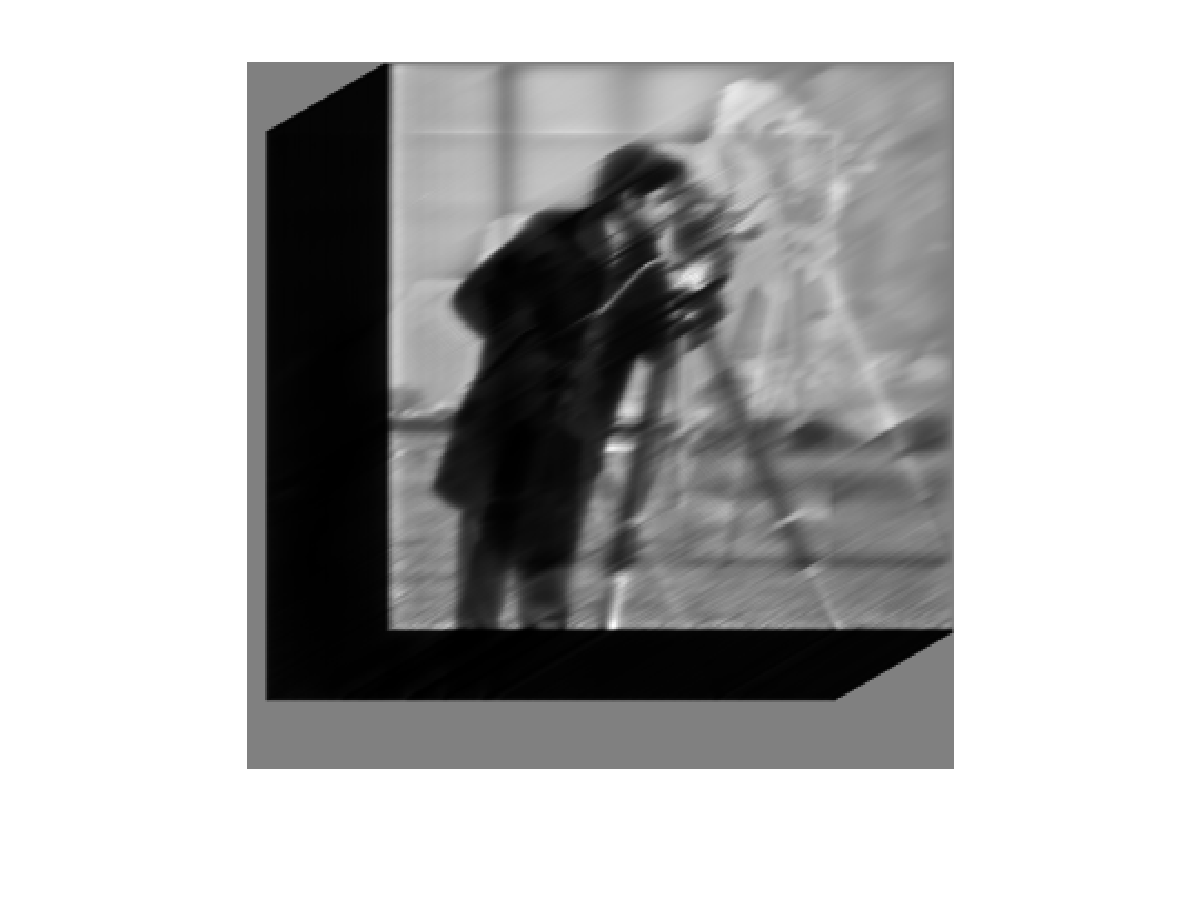
\includegraphics[width=0.9\textwidth]{cameraman-fullmagic-60_30-black.png}
\centering
\end{figure}
\vfill
\begin{minipage}{0.5\textwidth}
\begin{flushleft} \large
\emph{Group:} \\
3\\
~\\
\emph{Authors:}\\
Jonathan \textsc{Berthe} (XXX)\\
Arnaud \textsc{Cerckel} (45871100)\\
Benoit \textsc{Legat} (XXX)\\
Geoffroy \textsc{Vanderreydt} (XXX)\\
\end{flushleft}
\end{minipage}
\begin{minipage}{0.5\textwidth}
\begin{flushright} \large
\emph{Course:} \\
LFSAB 1507\\
~\\
\emph{Professors :} \\
Pierre-Antoine \textbf{Absil}\\
François \textbf{Glineur}\\
Julien \textbf{Hendrickx}\\
Yurii \textbf{Nesterov}\\
\emph{Assistants :}\\
Adrien \textbf{Taylor}\\
Adeline \textbf{Decuyper}
\end{flushright}
\end{minipage}
\vfill
\begin{center}
\begin{minipage}{0.25\textwidth}
\begin{flushleft}

\includegraphics[scale=0.25]{Couverture/ucl-logo.jpg}
\end{flushleft}
\end{minipage}
\begin{minipage}{0.48\textwidth}
\begin{center}
\Large{Academic year: 2013-2014}
\end{center}
\end{minipage}
\begin{minipage}{0.25\textwidth}
\begin{flushright}

\includegraphics[scale=0.5]{Couverture/epl-logo.jpg}
\end{flushright}
\end{minipage}
\end{center}
\end{titlepage}
\newpage


\section{Resources}
Mettez ici ce que vous trouvez intéressant
\begin{itemize}
  \item Montre comment trouver l'angle et la longueur en comparant Cepstral (mieux pour la longueur et mieux pour l'angle quand la longueur est petite (donc plus pour la caméra que pour le train)) et Radon (mieux pour l'angle avec une grande longueur donc pour le train) et Steerable filters (pourri) \cite{krahmer2006blind}.
    Explique aussi le problème du 45 degré où il faut renormaliser et de la fenêtre de Hann.
  \item Explication de Radon \cite{oliveira2007blind}.
  \item Angle: En gros, il faut voir l'angle des lignes qui sont dans le spectre pour ça il y a: Hough, Radon et Gabor et il conseille Gabor.
    Longueur: Il conseille d'utiliser un Cepstral modifié qu'on utilise et qui marche bien mieux \cite{Deshpande2014606}.
   \item  Rotational Motion Deblurring of a Rigid Object from a Single Image : pour la détection du foreground pour la caméra
   \item  Single Image Motion Deblurring Using Transparency: pour la détection du foreground pour la caméra
\end{itemize}

\section{Détermination de la PSF}
%\begin{figure}[!ht]
%  \centering
%  \begin{subfigure}[b]{0.45\textwidth}
%    \includegraphics[width=\textwidth]{onesFhot.png}
%    \caption{Transformée de fourier d'une image unitaire}
%    \label{fig:onesFhot}
%  \end{subfigure}
%  \begin{subfigure}[b]{0.35\textwidth}
%    \includegraphics[width=\textwidth]{cameramanFhot.png}
%    \caption{Transformée de fourier du caméraman flouté}
%    \label{fig:cameramanFhot}
%  \end{subfigure}%
%  \begin{subfigure}[b]{0.2\textwidth}
%    \includegraphics[trim=5cm 0cm 5cm 0cm, clip, width=\textwidth]{cameramanFhotradon.png}
%    \caption{Transformée de radon de la transformée de fourier du caméraman non-flouté}
%    \label{fig:cameramanFhotradon}
%  \end{subfigure}%
%  \begin{subfigure}[b]{0.4\textwidth}
%    \includegraphics[width=\textwidth]{cameramanvar.png}
%    \caption{Variance de la transformée de radon de la transformée de fourier du caméraman flouté}
%    \label{fig:cameramanvar}
%  \end{subfigure}
%  \caption{Tranformées de fourier}
%  \label{fig:fourier}
%  \begin{subfigure}[b]{0.35\textwidth}
%    \includegraphics[width=\textwidth]{cameramanBFhot.png}
%    \caption{Transformée de fourier du caméraman flouté}
%    \label{fig:cameramanBFhot}
%  \end{subfigure}%
%  \begin{subfigure}[b]{0.2\textwidth}
%    \includegraphics[trim=5cm 0cm 5cm 0cm, clip, width=\textwidth]{cameramanBFhotradon.png}
%    \caption{Transformée de radon de la transformée de fourier du caméraman flouté}
%    \label{fig:cameramanBFhotradon}
%  \end{subfigure}%
%  \begin{subfigure}[b]{0.4\textwidth}
%    \includegraphics[width=\textwidth]{cameramanBvar.png}
%    \caption{Variance de la transformée de radon de la transformée de fourier du caméraman flouté}
%    \label{fig:cameramanBvar}
%  \end{subfigure}
%  \caption{Tranformées de fourier}
%  \label{fig:fourier}
%\end{figure}

\subsection{Angle estimation}

\paragraph{Divers idées}
\begin{itemize}
  \item fft1
  \item rotate in time
  \item black around circle
  \item polar coordinate -> fft2 ou fft1
  \item radon en temporel
\end{itemize}

% TODO, refaire les images en floutant avec circular et en se souvenant de la longueur du flou...
Flouter, c'est faire une convolution en temporelle avec une marche,
ce qui fait une multiplication par $\frac{\sin(x)}{x}$ en fréquentiel.
Cette trace est assez visible.
En effet, sur la transformée de fourier de l'image de départ (figure~\ref{fig:cameramanvar}), il n'y a pas de trace visible alors
que lorsqu'on la floute, on obtient une trace à $\deg{70} + \deg{90}$ (le flou est à $(???, \deg{70})$).
Malheureusement, il y a aussi une croix qui se crée lorsqu'on floute qui est assez présente du fait qu'on a flouté avec ``replicate''.


\subsubsection{Var ou max}
Si on prend le cameraman qu'on tourne à \ang{45}, et qu'on floute à (40, \ang{10}), var donne \ang{3} et max donne \ang{10} !

\subsubsection{Problème de croix}
En \ang{0} et \ang{90}, il y a souvent une marque, indépendemment de l'angle, elles ressemblent même parfois à un $\sin(x)/x$ (voir la voiture de stivy tournée à \ang{45}~\ref{fig:car_cross} ou le cameraman flouté à (40, \ang{10}) tourné de \ang{45}).
C'est à se demandé si ce n'est pas du au fait qu'on prend un rectangle de l'image réel pour fft2
qui est un produit en temporel par deux passe-bas à \ang{0} et \ang{90}
(donc convolution par des $\sin(x)/x$ en fréquentiel ? Ici ça ressemble plus à un produit en fréquentiel...).
Serait-ce une bonne idée de passer en coordonnées polaires avant fft2 et faire fft2 sur l'image en polaire ?

%\begin{figure}[!ht]
%  \centering
%  \includegraphics[width=\textwidth]{car_cross.png}
%  \caption{Visible cross}
%  \label{fig:car_cross}
%\end{figure}

\subsubsection{Solutions}
On va ignorer un interval autour \ang{0} et \ang{90} pour éviter de fausser le calcul.
\paragraph{Première idée}
On prend de \ang{20} à \ang{70} (ainsi que \ang{110} à \ang{160}), puis on tourne l'image de \ang{45} et on refait pareil.
En suit, on prend le max sur tous les vars et si on trouve un de l'image tournée, on fait $-\ang{45}$ à l'angle trouvé.
Pour le cameraman à (40, \ang{10}), on a tout de même \ang{20}.

Le problème c'est que le pic à \ang{10} pour l'image non tournée est bien plus importante que celui à \ang{55} pour l'image trounée.
Du coup, même à \ang{20}, on a encore l'influence du pic.
Il ne faudrait pas se comparer les var ou max de l'original avec celle tournée de \ang{45} ou du moins, pas autant.

Il faudrait prendre le maximum de chaque image indépendemment et puis comparer.
Enfin, pour l'instant ça reste pareil mais si on fait le maximum pour les images séparément, on peut s'assurer qu'on est un pic et pas l'influence d'un pic.

\paragraph{Deuxième idée}
La méthode est la suivante.
\begin{itemize}
  \item Choisir le max de \ang{0} à \ang{179} qu'on nomme $a$.
    Si $a = \ang{0}$ ou $a = \ang{90}$ (éventuellement, plutôt $\max(|a - \ang{0}|, |a-\ang{90}|) < \epsilon$), il faudra trouver un autre $a$ en rognant.
  \item
    Alors tant que $a$ est \ang{0}, \ang{90} ou une valeur au bord d'un rognage (ou à un epsilon près),
    retirer $a$ de la liste des angles (ce qui la rogne).
    On lui rogne donc son début, sa fin (bah oui, si on met un epsilon, il faut aussi prendre 179 en compte ! :P) et son milieu.
\end{itemize}
On fait ça pour chaque orientation de l'image puis on compare la valeur pour les maxs trouvés (c'est ce que j'entends par ``pas autant'' comparer, on compare juste les maxs à la fin).

\chapter{Introduction)

Nowadays, more and more people deal with pictures, especially when they want to immortalize a special moment with their smartphone. But the pictures are often blurred because of a motion of the camera, the motion of a subject or a misfocus of the camera or for any other reason. That's why processing images, and especially deblurring, has become an important aspect in people's daily lives.

This report contains a study about the blur effect on an image and proposes some algorithms to remove that effect as much as possible. Blur can occur for many reasons. It is impossible to have a general method that solves all types of blur effects. That is why we only focus on two typical situations. In the first one, the picture has been taken from a moving train travelling with a known or unknown speed. In the second chosen situation, a security camera takes a picture with a moving subject. We dispose of several statistical images without any moving subject and we deblur the part of the image where we detected the moving subject.

The report begins with a clear and precise definition of what actually an image is and it gives a mathematical formulation for the blur problem. A good mathematical model of the blur effect is a key step in the understanding of this phenomena. Then extracting some information of the specified situation helps to get a more accurate model.

The mathematical modelisation is followed by the general strategy that we will follow to solve a deblurring problem. In this chapter, you will encounter our special item that we wanted to focus on: fast computing. Even if the main goal of this report is to achieve good results of deblurring, we also treated the case where the quickiness is more important than the quality. This especially applies on the situation with the security camera. For example, a security man observes the images of a camera in a room on his screen. He only needs an idea of what is going on in the room but right now, on this moment and not 1 hour ago.

Subsequently, we go in a deeper analysis of what is described in the general strategy. We explain the methods we use to deblur and compare them for different images and different types of blur.

Finally, we end with the strengths and the weaknesses of this project and some suggested improvements. A conclusion resumes the main point of this report. All the algorithms have been implemented with \texttt{Matlab} and the codes have been included in the appendices.
\label{mathModel}
% TODO explain that int_x int_y h(x,y) dx dy = 1 
\section{What is an image?}

An image is a two dimensional signal $f(x,y)$ that takes the position of a point on a plan as argument and returns the luminance intensity at that point. If the image is gray-scaled, the output is a scalar:
\begin{eqnarray}
f:\Omega \rightarrow \mathbb{R}: (x,y) \mapsto f(x,y),
\end{eqnarray}
where $\Omega \subseteq \mathbb{R}^2$. If we have a coloured image, we adopt a RGB (Red-Green-Blue) representation and the output will be 3-dimensional (one dimension per primitive colour):
\begin{eqnarray}
f:\Omega \rightarrow \mathbb{R}^3 : (x,y) \mapsto f(x,y).
\end{eqnarray}
Along this report, we will only consider gray-scaled images but we can easily generalize the problem to coloured images. $f$ is a continuous signal. But to be able to manipulate an image, we will often have to discretize this signal. The discretized signal is then of the form $f(m,n)$, where $m=1...M$ and $n=1...N$ with $M,N \in \mathbb{N}_0$. The signal can then be represented by a matrix $F$ (3 matrices for coloured images). An element  of this matrix is called a pixel. The values of $f(m,n)$ are often represented by words of $8$ bits so $f(m,n)$ can take $256$ different values: $f(m,n) \in \left[0...255\right]$.

\section{What is blurring?}

Blurring is the operation of mixing the spatial information of an image. In this section, we will try to give an accurate description of a continuous model and a discrete model for blurring.

\subsection{Continuous model}

Let $\mathcal{H}$ denote the operator of blurring. If $f(x,y)$ is the original image and $g(x,y)$ the blurred version of it, then we can represent the operation of blurring by the system shown on figure $(\ref{system})$ or by the following equation:
\begin{equation}
g(x,y) = \mathcal{H}\left\lbrace f(x,y) \right\rbrace.
\end{equation}

\begin{figure}
\begin{center}
\begin{tikzpicture}[every text node part/.style={align=center}, every node/.style={scale=0.7},scale=0.7]

\draw(3,0)--(7,0)--(7,3)--(3,3)--(3,0);

\draw(5,1.5)node{blur \\ $\mathcal{H}$};

\draw[->](0,1.5)--(3,1.5);
\draw[->](7,1.5)--(10,1.5);

\draw(0,1.5)node[above]{$f(x,y)$};
\draw(10,1.5)node[above]{$g(x,y)$};

\end{tikzpicture}
\end{center}
\caption{System representation of blurring}
\label{system}
\end{figure}

We suppose the blurring operator to be linear. This assumption will be verified in the specific situations we have chosen (train and camera). Mathematically, we write:
\begin{equation}
\mathcal{H}\left\lbrace \alpha f_1(x,y) + \beta f_2(x,y) \right\rbrace =  \alpha \mathcal{H}\left\lbrace f_1(x,y)\right\rbrace + \beta \mathcal{H}\left\lbrace f_2(x,y)\right\rbrace,
\end{equation}
for $\alpha, \beta \in \mathbb{R}$.
Secondly, we may assume the operator is shift-invariant: when the input signal is shifted, the output signal is shifted by the same amount. This implies that the blurring system responds identically, no matter where on the plan the input is applied, which seems intuitively correct for images where all the objects of the scene are approximatively on the same vertical plane (this is an assumption we will make in the specific situations, cfr. infra). Mathematically:

if $\mathcal{H}\left\lbrace f(x,y) \right\rbrace = g(x,y)$, then $\mathcal{H}\left\lbrace f(x-x_0,y-y_0) \right\rbrace = g(x-x_0,y-y_0)$.

The input signal can be represented by a weighted superposition of shifted impulses \cite{haykin2007signals}. Because of the linearity of the system, the output is a weighted superposition of the responses of the system to each shifted impulse. The system is also shift-invariant so the system's response to a shifted impulse is a shifted version of the system's response to an impulse. Hence, the output is given by a weighted superposition of shifted impulse responses. This weighted superposition is called $\emph{convolution}$. So, if $f(x,y)$ is the input, $h(x,y)=\mathcal{H}\left\lbrace \delta(x,y) \right\rbrace$ ($\delta(x,y)$ is an impulse signal) is the system's impulse response and $g(x,y)$ is the output, then we write:
\begin{eqnarray}
g(x,y) &=& \mathcal{H}\left\lbrace f(x,y) \right\rbrace \\
g(x,y) &=& h(x,y) \ast f(x,y),
\end{eqnarray}
where $\ast$ is the convolution symbol. So blurring is spreading the value of a pixel by a certain way which is determined by $h$. That's why we call $h$ also the Point Spread Function (PSF).

When we take a picture, the image that we get is usually affected by additive noise. Additive means that the noise does not depend on the input signal. If $e(x,y)$ denotes the additive noise, we can represent the system by the scheme  given in figure $(\ref{systemnoise})$ or by the following equation:
\begin{eqnarray}
g(x,y) &=& \mathcal{H}\left\lbrace f(x,y) \right\rbrace + e(x,y) \\
 &=& f(x,y) \ast h(x,y) + e(x,y).
\label{generaleq}
\end{eqnarray}
This noise represents measurement and round-off errors and also errors due to the model (convolution) we use to represent blurring.

\begin{figure}
\begin{center}
\begin{tikzpicture}[every text node part/.style={align=center}, every node/.style={scale=0.7},scale=0.7]

\draw(3,0)--(7,0)--(7,3)--(3,3)--(3,0);
\draw(5,1.5)node{blur \\ $\mathcal{H}$};

\draw(10.5,1.5)circle(0.5);
\draw(10.5,1.5)node{$+$};

\draw[->](0,1.5)--(3,1.5);
\draw[->](7,1.5)--(10,1.5);
\draw[->](10.5,5)--(10.5,2);
\draw[->](11,1.5)--(14,1.5);

\draw(0,1.5)node[above]{$f(x,y)$};
\draw(14,1.5)node[above]{$g(x,y)$};
\draw(10.5,5)node[right]{$n(x,y)$};

\end{tikzpicture}
\end{center}
\caption{System representation of blurring with noise}
\label{systemnoise}
\end{figure}


\subsection{Discrete model}

Like we said earlier, in the discrete model, the signals can be represented by matrices. The operation of $\mathcal{H}$ on $f$ can then be replaced by a matrix multiplication of $H \in \mathbb{R}^{M \times M}$ (the matrix associated with the operator $\mathcal{H}$) with $F \in \mathbb{N}^{M \times N}$ (the matrix associated with the input signal $f$). Equation $(\ref{generaleq})$ becomes:
\begin{equation}
G = HF + E,
\label{eqmatrix}
\end{equation}
where $E \in \mathbb{R}^{M \times N}$ is the matrix associated with the additive noise $e$. To handle this problem more easily, we would like to solve a linear system. That's why we are going to make a vector of a matrix representing an image. So if $F \in \mathbb{N}^{M \times N}$ is a matrix representing an image, then the corresponding vector $\mathpzc{f} = vec(F) \in \mathbb{N}^{MN \times 1}$ is constructed by putting the columns of $F$ under each other. Watch out for the notation used: $f$ is a continuous signal, $F$ is the matrix associated with this signal and $\mathpzc{f}$  is the vector corresponding to this matrix. Equation $(\ref{eqmatrix})$ becomes:
\begin{equation}
\mathpzc{g} = \tilde{H}\mathpzc{f} + \mathpzc{e},
\label{eqvec}
\end{equation}
where $\tilde{H} \in \mathbb{R}^{mn \times mn}$ is the result of the following Kronecker product:
\begin{equation}
\tilde{H} = I_n \otimes H,
\end{equation}
with $I_N$ the identity matrix of dimension $N$. By equation $(\ref{eqvec})$, we clearly see that a pixel of the blurred image is a linear combination of pixels of the original image, plus some noise. In the following section, we will always take the matrix form of an image but the vector form can be easily get by the equations just above.

\section{What is deblurring?}

Deblurring is the inverse operation of blurring. So it consists in getting an approximation of the image $\mathpzc{f}$ from the blurred image $\mathpzc{g}$ by solving equation $(\ref{eqvec})$. Due to the noise, this problem is not well-posed so we try to solve the following optimization problem \footnote{In equation $(\ref{eqmin})$ we omitted the tilde to ease the notation.}
\begin{equation}
min_{\mathpzc{f}} ||H\mathpzc{f}-(\mathpzc{g}-\mathpzc{e})||^2.
\label{eqmin}
\end{equation}
But if $H$ is ill-conditioned or singular, we need to add regularization terms. We use here the Tikhonov regularization:
\begin{equation}
min_{\mathpzc{f}} ||H\mathpzc{f}-(\mathpzc{g}-\mathpzc{e})||^2+||\Gamma \mathpzc{g}||^2,
\end{equation}
for some suitable chosen Tikhonov matrix $\Gamma$. Until now we always assumed $H$ was known but in a real situation we only know $\mathpzc{f}$ and nothing about $H$. That's why we approximate $H$ based on some information about how the image has been blurred. Finding this approximation is the subject of the following section.

\section{Specific situations}

Like we said in the previous section, to approximate the blurring operator, we need some information on the reason why the image has been blurred. We have chosen two typical situations in which blur effect occur. The first one is a picture that has been taken from a moving train wtih known or unknown speed. The second one is a picture depicted by a security camera. The goal is to deblur the part of the image where a subject is moving. We also dispose of several statistical images without the subject.

\subsection{Train}

First we need to make some assumptions about the circumstances to get an idea of what $H$ should look like. We assume that the picture has been taken with the camera parallel to the train (hyp. 1). This means that the blur effect will only appear horizontally on the picture. We also assume that the speed of the train is constant during the short period of time when the picture is taken (hyp. 2). This allows us to suppose the blurring operator to be linear: every pixel is modified in the same way. If the speed isn't constant, the parts of the image where the camera is going faster, are influenced by more pixels then the parts where the camera is going slower. The operation is not linear anymore and we won't take this case into account. We will first treat the case where the speed of the train is known and then when it is unknown. Finally we suppose the subjects on the picture to be in the same vertical plane (hyp. 3). So every subject lies approximatively on the same distance away from the camera. This also means that blurring will approximatively have the same effect everywhere on the image. If this was not the case, the blur effect would be more visible on subjects near the camera.

Based on all those assumptions, we can now build an approximative form for the blurring matrix $H$. So we have to answer to the following question: ``How is a pixel of $G$ constructed based on the pixels of $F$?''. Through hypothesis 2, we know that only the pixels belonging to the same row as the pixel of $G$ that we are studying, will influence that pixel. If the train is travelling to the left (respectively to the right), a certain number of pixels on the right (respectively left) of that pixel will influence it. Let's denote this number of pixels by $k$. By linearity, we can say that the blurred image is a weighted superposition of shifted versions of the original image. If $D$ is a matrix representing the operator that shifts the image by one pixel horizontally, we can define the blurring matrix $H$ as:
\begin{equation}
H=\sum\limits_{i=0}^{k} c_i D^{i}.
\label{eqHtrain}
\end{equation}

Now we still have to determine $k$ and the factors $c_i \in \mathbb{R}$ based on the assumptions we made. Let's begin by $k$. If the speed is unknown, we cannot find an analytical representation for $k$. This case will be treated in later chapters. So for now, we suppose the speed of the train known and denote it by $v$. Intuitively, we expect $k$ to be increasing when the speed or the opening time also does. On the opposite, $k$ should decrease when the average distance goes up. We already mentioned that before. If $\phi$ is the opening angle of the camera and $\eta$ is the average distance from the camera to the scene, we can represent the situation by figure \ref{situation}. The width $W$ of the scene is then obtained by: 
\begin{equation}
W = 2 \eta \tan\left(\frac{\phi}{2}\right).
\end{equation}
A row of the matrix associated to the image $F$ represents then a real line of length $W$. If $F$ has $N$ columns, the width of one pixel $W_e$ is
\begin{eqnarray}
W_e &=& \frac{W}{N} \\
&=& \frac{2 \eta }{N}\tan\left(\frac{\phi}{2}\right).
\end{eqnarray}
We now want to know the time it takes to a real segment of length $W_e$ to be represented by the next pixel. We denote this time by $\Delta t_e$ and we get:
\begin{eqnarray}
\Delta t_e &=&\frac{W_e}{v}\\
&=& \frac{2 \eta }{Nv}\tan\left(\frac{\phi}{2}\right).
\end{eqnarray}
Finally, we compute $k$ knowing that it is the number of times $\Delta t_e$ can be put in the opening time $\Delta t$ of the camera:
\begin{eqnarray}
k &=& \frac{\Delta t}{\Delta t _e} \\
&=& \dfrac{Nv\Delta t}{2 \eta \tan\left(\frac{\phi}{2}\right)}.
\end{eqnarray}

From this equation, we can verify our expectations: $k$ is proportional to $v$ and $\Delta t$, and inversely proportional to $\eta$.

\begin{figure}
\begin{center}
\begin{tikzpicture}[every text node part/.style={align=center}, every node/.style={scale=0.7},scale=0.7]

\draw(0,0)--(3,0)--(1.5,-6)--(0,0);
\draw[<->](3.5,0)--(3.5,-6);
\draw[<->](0,0.5)--(3,0.5);

\draw(1.5,0.5)node[above]{$W$};
\draw(3.5,-3)node[right]{$\eta$};
\draw(1.5,-5)node{$\phi$};

\end{tikzpicture}
\end{center}
\caption{Representation of the situation when the picture is taken.}
\label{situation}
\end{figure}

Now what about the coefficients $c_i$? Let's suppose the train is travelling to the right, so a pixel $G(m,n)$ is a weighted sum of the $k$ pixels to the left of the corresponding pixel $F(m,n)$ (plus itself). As the speed of the train is constant, every weight should be equal. Pixels of $G$ also have a range from $0$ to $255$ so the weighted sum must not exceed the maximum. That's why we have $c_i=\frac{1}{k+1}$.

The last thing we need to determine in  equation $(\ref{eqHtrain})$ is the matrix $D$. A first version of it for a $3 \times 3$ image could be (we are still considering the train is moving to the right):
$$
\begin{pmatrix}
a & b & c \\
c & d & e \\
f & g & h \\
\end{pmatrix}
\begin{pmatrix}
0 & 1 & 0 \\
0 & 0 & 1 \\
0 & 0 & 0
\end{pmatrix}
=
\begin{pmatrix}
0 & a & b \\
0 & c & d \\
0 & f & g \\
\end{pmatrix}.
$$
Suppose we model the blurring of this $3 \times 3$ matrix $F$ with $k=1$ (we neglect the noise effect). We then have $G(i,3) = \frac{1}{2} F(i,2) + \frac{1}{2} F(i,3)$ for $i={1,2,3}$, just like we expected. It also works for the second column. But for the first column, we get: $G(i,1) = \frac{1}{2} F(i,1$ for $i={1,2,3}$, so it only makes the left border of the original image darker (as 0 is black and 255 is white). If we took a bigger $k$, we would observe this for all the columns for which $n \leq k$ as they need some information out of the image. Actually, with this matrix $D$, we considered that everything that is beyond the scope of the image is black, and that is of course a bad approximation. So to get a better information about what is beyond the left edge of the image, we could approximate it by extrapolation. A simple example is the polynomial extrapolation of order 0. This consists in putting the first column $k$ times on the left of the image. Using the same example, we get:
$$
\begin{pmatrix}
a & b & c \\
c & d & e \\
f & g & h \\
\end{pmatrix}
\begin{pmatrix}
1 & 1 & 0 \\
0 & 0 & 1 \\
0 & 0 & 0
\end{pmatrix}
=
\begin{pmatrix}
a & a & b \\
c & c & d \\
f & f & g \\
\end{pmatrix}.
$$
Now we have : $G(i,1) = F(i,1)$ for $i={1,2,3}$, which is a little bit better than the previous model. If we take a higher order of extrapolation, we get a better approximation of the real blurring effect.

%TODO pas compris le truc avec le C_1-j pour l'extrapolation d'ordre 1

Another way to treat those ``edge problems'' is by modelling the blur effect on a smaller image. If we apply our model on the image defined by $F_{small} = F(m,n)$ for $m>k$, then we have all the ``missing information'' and we don't need to extrapalte anymore.


\subsection{Security camera}

Our next situation is a fixed camera taking a sample of pictures with everytime the same scene but sometimes disturbed by a person walking around. The goal is to deblur the part of the image where a person is walking. There are three differences compared to the situation with the train. Firstly, only a part of the image is blurred, so deblurring will also be only applied on that part. Moreover, if the person is not too close to the edges of the image, we don't have any ``edge problems'' anymore. And finally, the person could walk in any direction so we don't have a perfect horizontal blur effect anymore.

Now how can we detect a walking person on an image? If we have a high number of statistical images, we can build a background-image that contains the average value of each pixel. If we take the difference between the blurred image and this image, we get an image that contains very small values (near to zero) for the regions where the person is not present and bigger values for the regions that we call the foreground. Next we extract the foreground and we deblur this new image.

\chapter{General strategy}
\section{Train}
Let's summarize the model.
We know $g(x,y)$ and we know that there is a $h(x,y)$ such that
\[ g(x,y) = h(x,y) * f(x,y) + e(x,y). \]
We would like to find $f(x,y)$.
To obtain it, we need to deconvolve $g(x,y)$ with a method
robust to the noise $e(x,y)$.

However, we don't know $h(x,y)$ so we first need to estimate it
in a way that is also robust to the noise.
It is easier to estimate $h(x,y)$ if we make some assumptions.
For our problem, we have a motion blur which means that
$h(x,y)$ only depends on an angle and a length which are
respectively the angle at which the blur is and the number of
pixel on which each pixel depends.

Once we have an estimate of $h(x,y)$, we then deconvolve
$g(x,y)$ to get an estimate $\hat{f}(x,y)$.
For some deconvolution method, we need an estimate of
some properties of the noise which is done only using $g(x,y)$.

\section{Camera}
On the camera case, we have a serie of images.
The images are obtained from a fixed camera capturing a fixed
background with some objects appearing in some images.
\begin{enumerate}
  \item For the first images, we only estimate the background.
    The background is obtained as the mean of the pixels,
    we also calculate the variance.
  \item For each following images, we use the background and the variance
    to detect the foreground.
    We take the ``biggest'' connected shape and then deblur it.
    Once it is deblurred, we put it back on the background.
  \item We can then update the background.
    Indeed, if for example, a chair is added to the background
    or the light is changing, we need the background to be updated.
    The mean is then not exactly the mean nor the variance
    since we wand new images to have more importance than previous
    images.
\end{enumerate}

\section{Estimation of the PSF}
\subsection{angle estimation with the Gabor filter}

The Gabor filter is a gaussian filter modulated by a sinusoidal wave. The function of this filter is given by:
\begin{equation}
B(x,y)=dfrac{1}{2\pi \sigma_x \sigma_y} exp\left[-\frac{1}{2}\left(\frac{x^2}{\sigma_x^2}+ \frac{y^2}{\sigma_y^2} \right) -j\omega(xcos\phi + ycos\phi)\right],
\label{filtreGabor}
\end{equation}
where $\sigma_x$ and $\sigma_y$ are the standard deviations in the $x$ and $y$ directions. The parameters $\phi$ and $\omega$ are the direction and the frequency of the filter respectively. Only $\phi$ will vary while the other parameters stay fixed. According to the article (?? ref dash20.. ??), experimentation has shown that good values for $\sigma$ and $\omega$ are $3$ and $1.75$ respectively. The method consists in applying the Gabor filter to the power spectrum of the blurred image and then detecting the blur angle $\theta_{blur}$ by searching for the $\phi$ that gives the highest response value. This value can be calculated using $L_2$ norm. The $\phi$ obtained by this method is the blur angle. Here are the steps of the algorithm:

1. computation of the spectrum of the blurred image by a two dimensional Fourier transform\\
2. taking the logarithm of it\\
3. convolving this with the Gabor function given by equation $(\ref{filtreGabor})$ for different $\phi$, the result is $R(\phi)$\\
4. for every $\phi$, taking the $L_2$ norm: $||R(\phi)||$
5. the blur angle is the parameter $phi$ that gives the biggest norm:
\begin{equation}
\theta_{blur} = arg \left\lbrace max_{\phi}R(\phi)\right\rbrace.
\end{equation}

This algorithm is implemented by our matlab function $angle_estimator_Gabor(f,thetamin, thetamax)$, where the input $f$ is the blurred image. The parameter $\phi$ will vary from $thetamin$ to $thetamax$. If those inputs are not specified, we set them to $0$ for $thetamin$ and $180$ for $thetamax$.

%TODO Resultats en images



\section[Deconvolut.]{Deconvolution}

\section[Compl. Treatment]{Complementary Treatment}
\begin{frame}
  \frametitle{no referential blur metric}
  
  advantage: absolute metric, no need of the original image\\
  steps:
  \begin{itemize}
  \item vertical edges (Sobel)
  \item analysing the image image by row. Everytime a pixel that is part of an edge is found, determining the local minimum and extremum on that row.
  \item local blur = distance (in pixels) between the extrema
  \item global blur = average of local blurs
  \end{itemize}
\end{frame}
\section{Adaptations for camera}

\begin{frame}
	\frametitle{Background estimation}
	\begin{enumerate}
	\item Input: $k$ images (size $M$x$N$ for gray-scaled image) from fixed camera
	\item Output: Matrix M (size $M$x$N$). In (m,n), means  of the k images only if ($i = 1,\cdots, k)$:	
	$$I_i (m,n) \in [med(m,n) - Inter(m,n); med(m,n) + Inter(m,n)]$$
    \item Exemples
	\end{enumerate}

\begin{figure}[h]
\centering
\begin{subfigure}{0.20\textwidth}
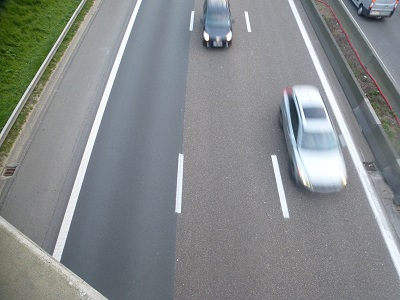
\includegraphics[width= \textwidth]{../Images/Camera/Autoroute/fg/06.jpg}
\caption{}
\label{fig:Aut1}
\end{subfigure}
~
\begin{subfigure}{0.20\textwidth}
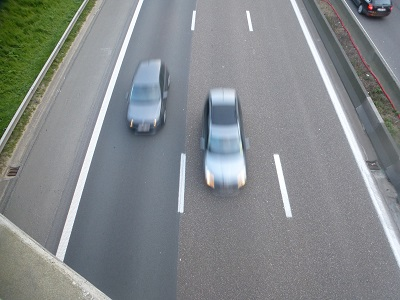
\includegraphics[{width= \textwidth}]{../Images/Camera/Autoroute/fg/07.jpg}
\caption{}
\label{fig:Aut2}
\end{subfigure}
~
\begin{subfigure}{0.20\textwidth}
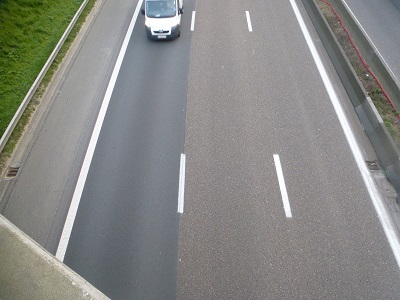
\includegraphics[{width= \textwidth}]{../Images/Camera/Autoroute/fg/08.jpg}
\caption{}
\label{fig:Aut3}
\end{subfigure}
~
\begin{subfigure}{0.20\textwidth}
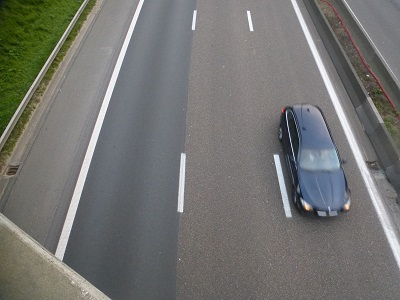
\includegraphics[{width= \textwidth}]{../Images/Camera/Autoroute/fg/09.jpg}
\caption{}
\label{fig:Aut4}
\end{subfigure}
~
\begin{subfigure}{0.20\textwidth}
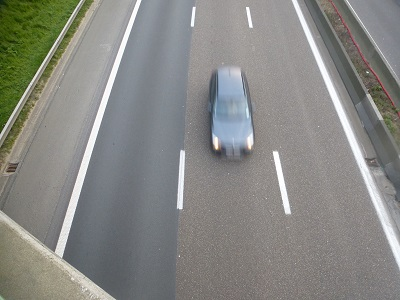
\includegraphics[{width= \textwidth}]{../Images/Camera/Autoroute/fg/10.jpg}
\caption{}
\label{fig:Aut5}
\end{subfigure}
~
\begin{subfigure}{0.20\textwidth}
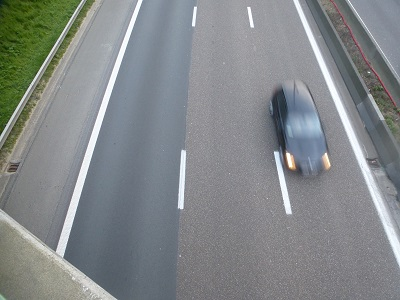
\includegraphics[{width= \textwidth}]{../Images/Camera/Autoroute/fg/11.jpg}
\caption{}
\label{fig:Aut6}
\end{subfigure}
~
\begin{subfigure}{0.20\textwidth}
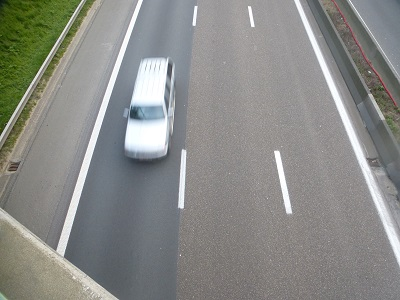
\includegraphics[{width= \textwidth}]{../Images/Camera/Autoroute/fg/12.jpg}
\caption{}
\label{fig:Aut7}
\end{subfigure}
~
\begin{subfigure}{0.20\textwidth}
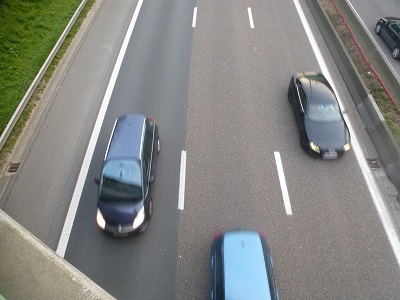
\includegraphics[{width= \textwidth}]{../Images/Camera/Autoroute/fg/13.jpg}
\caption{}
\label{fig:Aut8}
\end{subfigure}
~
\begin{subfigure}{0.20\textwidth}
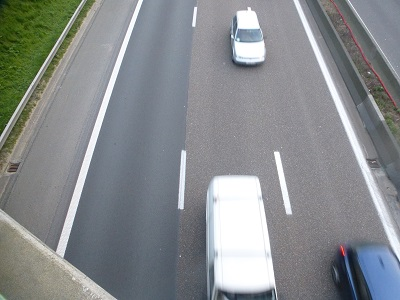
\includegraphics[{width= \textwidth}]{../Images/Camera/Autoroute/fg/14.jpg}
\caption{}
\label{fig:Aut9}
\end{subfigure}
~
\begin{subfigure}{0.20\textwidth}
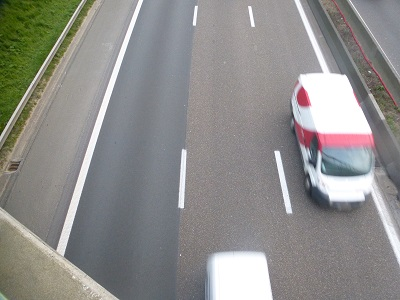
\includegraphics[{width= \textwidth}]{../Images/Camera/Autoroute/fg/15.jpg}
\caption{}
\label{Aut10}
\end{subfigure}
~
\begin{subfigure}{0.20\textwidth}
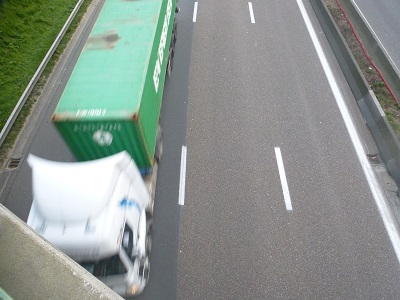
\includegraphics[{width= \textwidth}]{../Images/Camera/Autoroute/fg/16.jpg}
\caption{}
\label{fig:Aut11}
\end{subfigure}
\caption{Images taken by camera video}
\label{fig:AllAut}
\end{figure}

\begin{figure}[h]
\centering
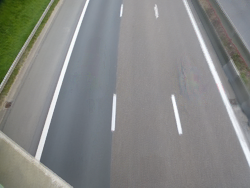
\includegraphics[{width=0.4 \textwidth}]{../Images/Camera/Autoroute/BGDetect/BGDetect.png}
\caption{Background estimation}
\label{fig:AutBG} 
\end{figure} 

\begin{frame}
	\frametitle{: Update of the background}
	\begin{enumerate}
	\item Formula
	$$I_i (m,n) \in [med(m,n) - Inter(m,n); med(m,n) + Inter(m,n)]$$
	Typically, $a = 0.99$
	\item Exemples with $a = 0.5$
	
\begin{figure}[h]
\begin{figure}[h]

\centering
\begin{subfigure}{0.20\textwidth}
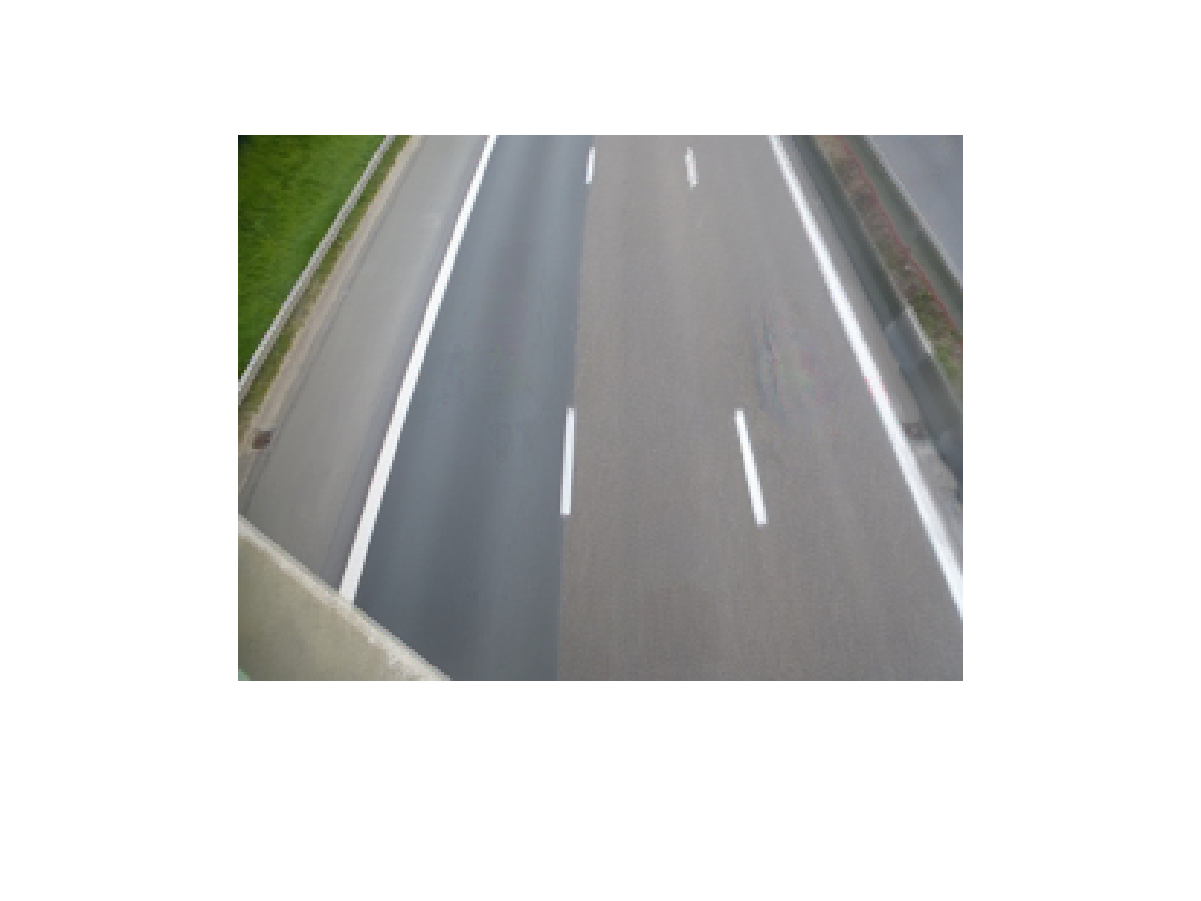
\includegraphics[width= \textwidth]{../Images/Camera/Autoroute/fg/a50/CamDeblurred-1.png}
\caption{}
\label{fig:UAut1}
\end{subfigure}
~
\begin{subfigure}{0.20\textwidth}
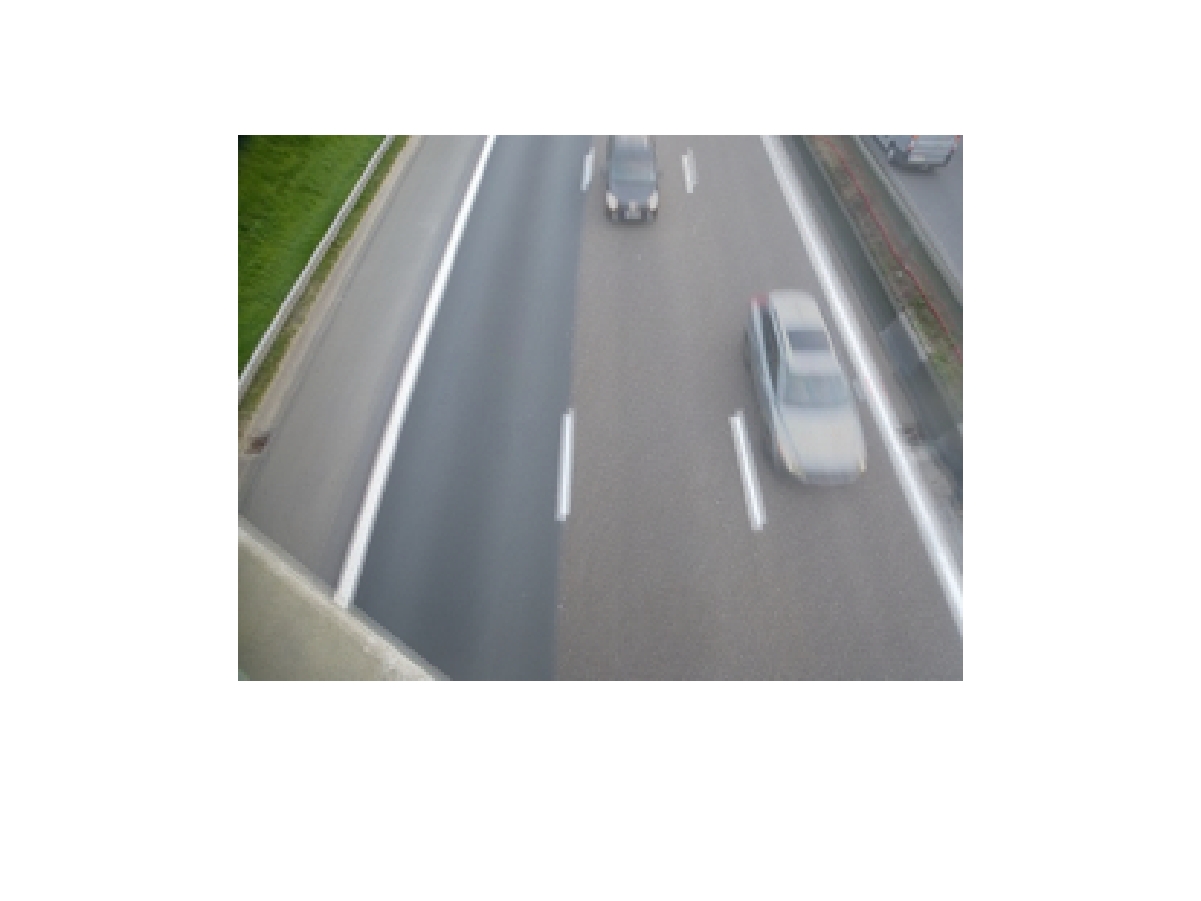
\includegraphics[{width= \textwidth}]{../Images/Camera/Autoroute/fg/a50/CamDeblurred-2.png}
\caption{}
\label{fig:UAut2}
\end{subfigure}
~
\begin{subfigure}{0.20\textwidth}
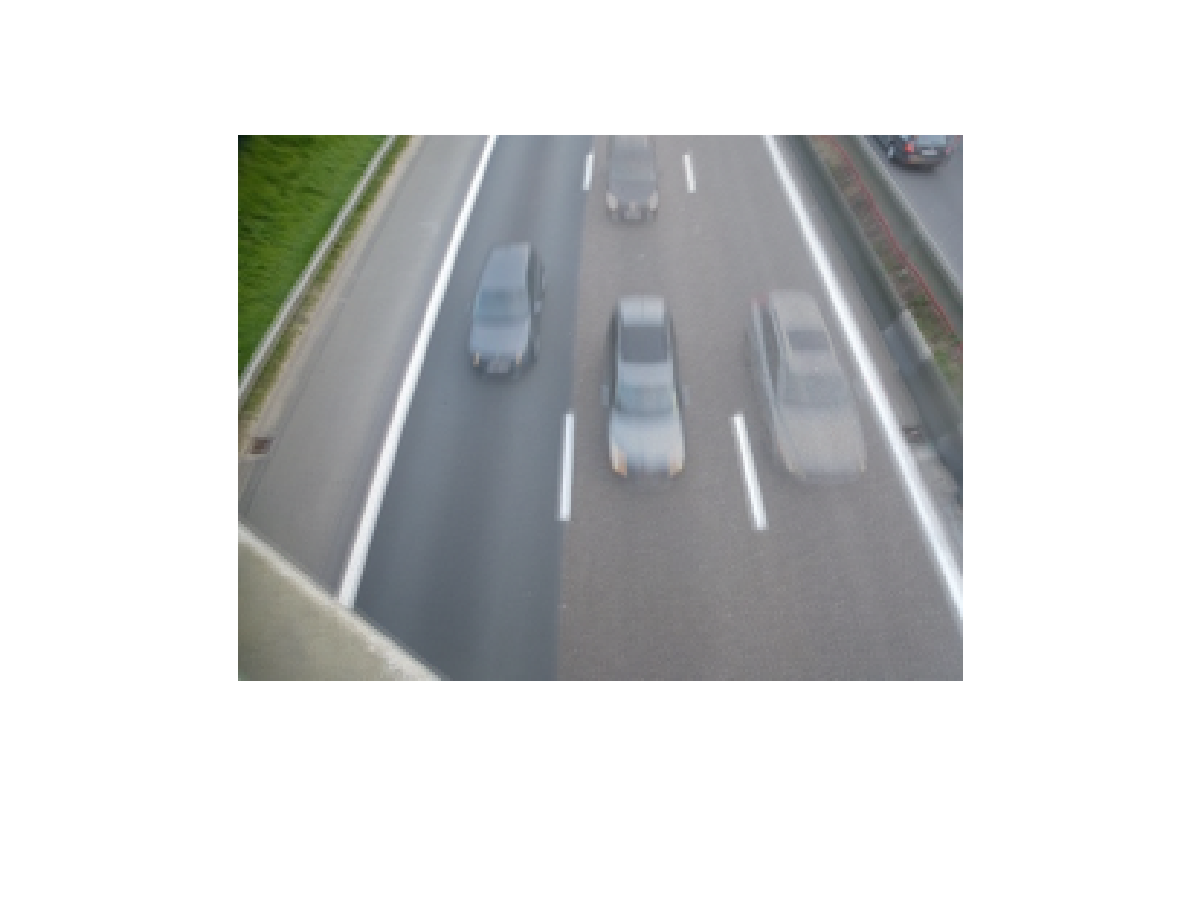
\includegraphics[{width= \textwidth}]{../Images/Camera/Autoroute/fg/a50/CamDeblurred-3.png}
\caption{}
\label{fig:UAut3}
\end{subfigure}
~
\begin{subfigure}{0.20\textwidth}
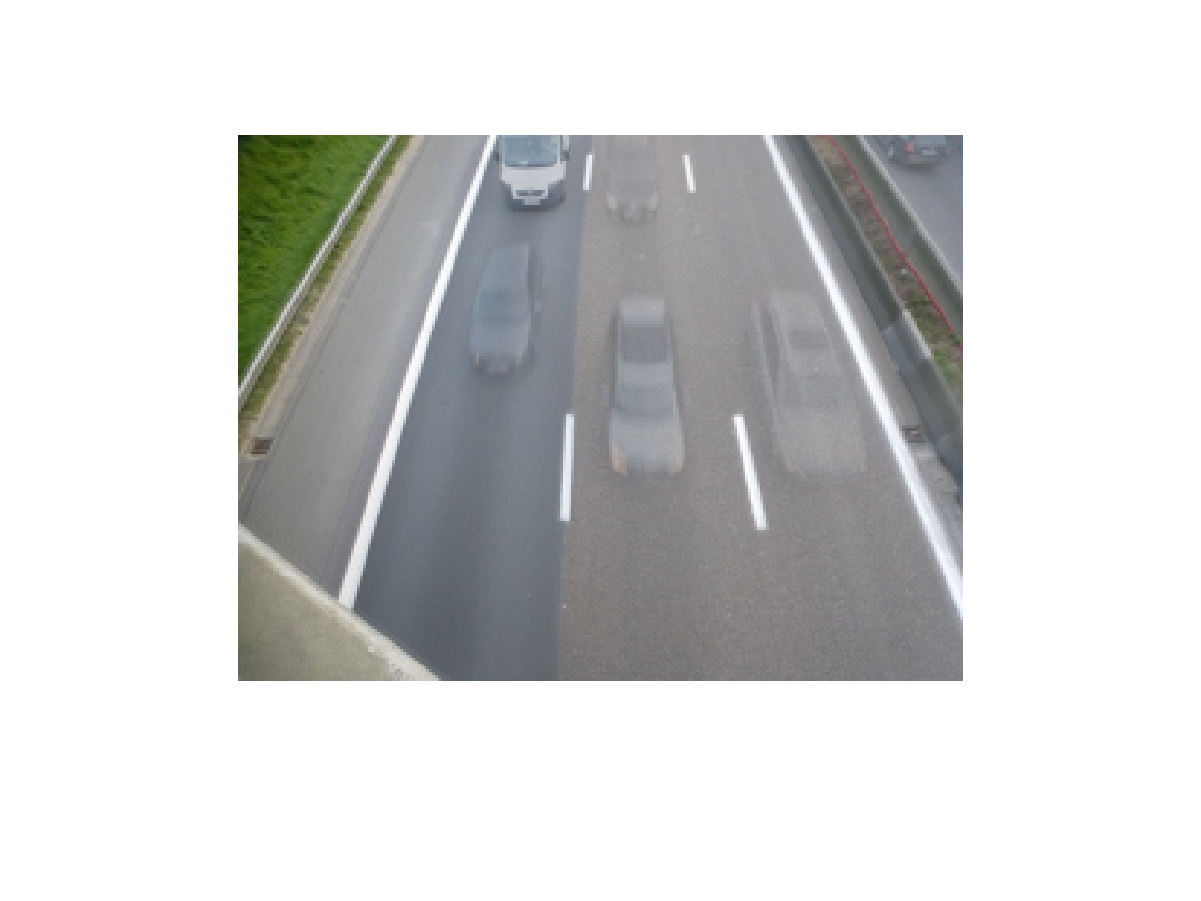
\includegraphics[{width= \textwidth}]{../Images/Camera/Autoroute/fg/a50/CamDeblurred-4.png}
\caption{}
\label{fig:UAut4}
\end{subfigure}
~
\begin{subfigure}{0.20\textwidth}
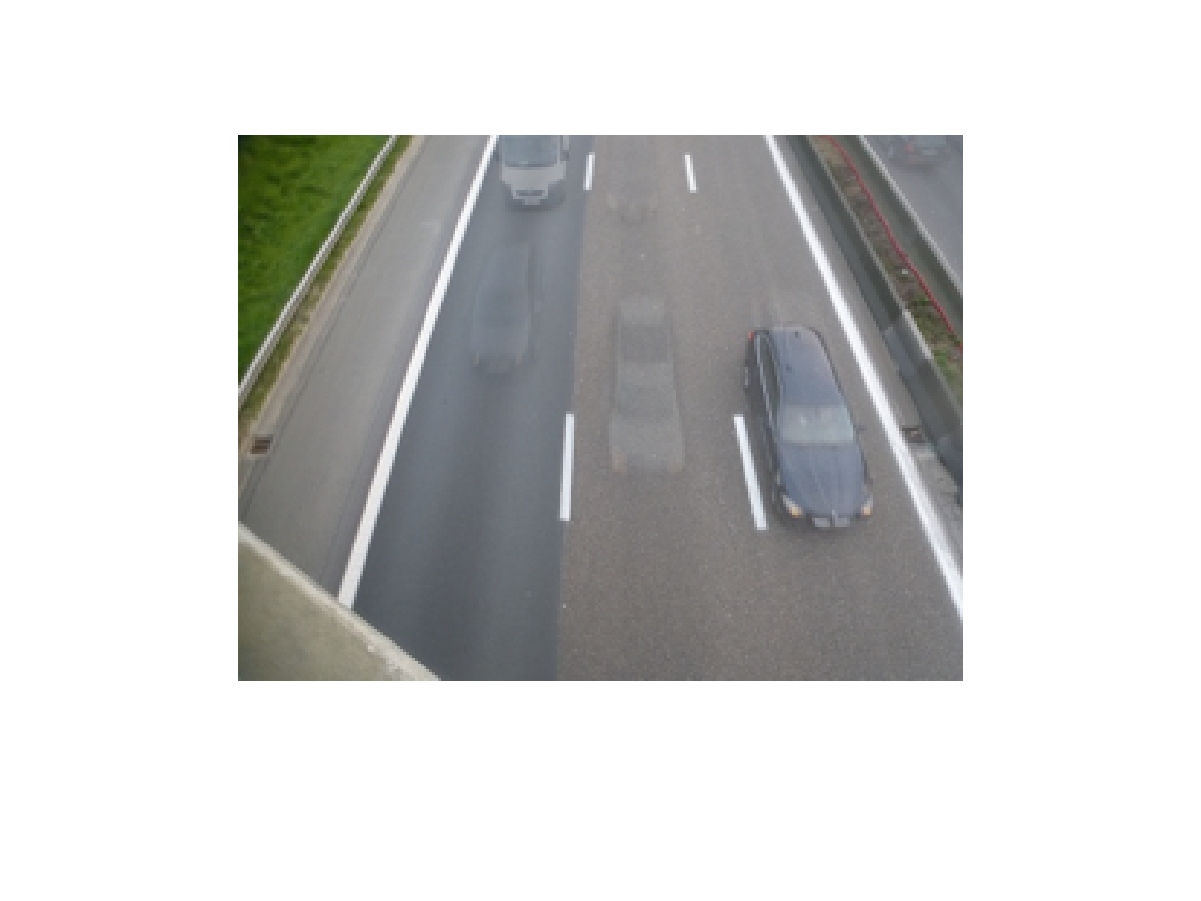
\includegraphics[{width= \textwidth}]{../Images/Camera/Autoroute/fg/a50/CamDeblurred-5.png}
\caption{}
\label{fig:UAut5}
\end{subfigure}
~
\begin{subfigure}{0.20\textwidth}
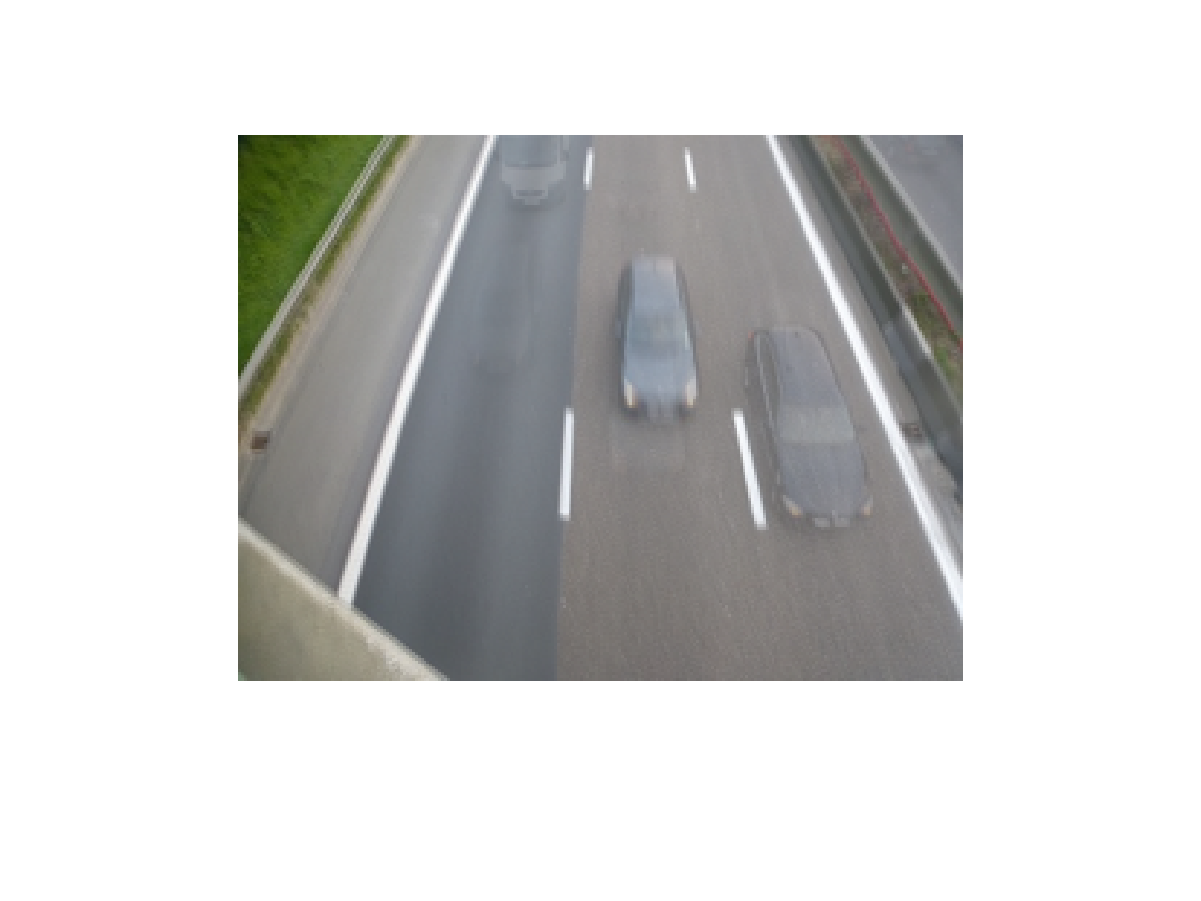
\includegraphics[{width= \textwidth}]{../Images/Camera/Autoroute/fg/a50/CamDeblurred-6.png}
\caption{}
\label{fig:UAut6}
\end{subfigure}
~
\begin{subfigure}{0.20\textwidth}
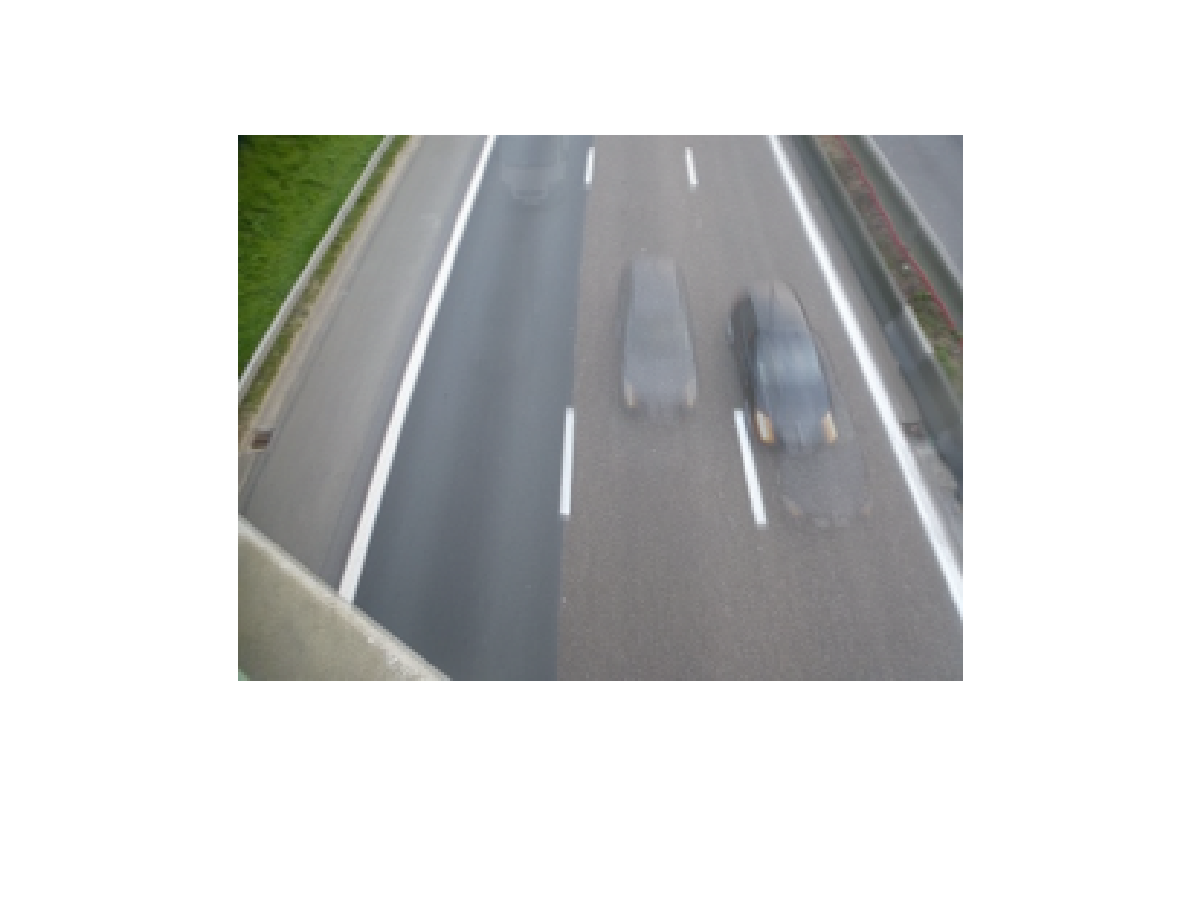
\includegraphics[{width= \textwidth}]{../Images/Camera/Autoroute/fg/a50/CamDeblurred-7.png}
\caption{}
\label{fig:UAut7}
\end{subfigure}
~
\begin{subfigure}{0.20\textwidth}
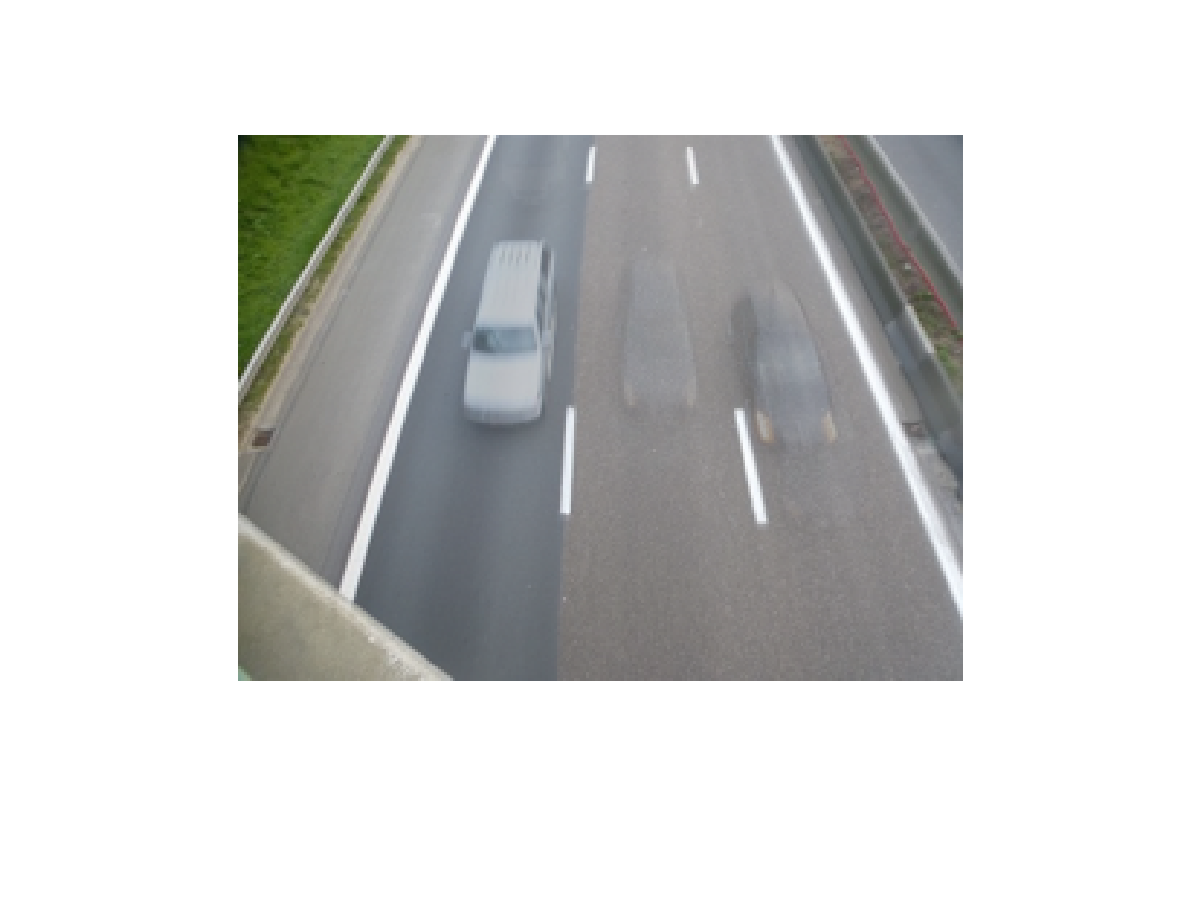
\includegraphics[{width= \textwidth}]{../Images/Camera/Autoroute/fg/a50/CamDeblurred-8.png}
\caption{}
\label{fig:UAut8}
\end{subfigure}
~
\begin{subfigure}{0.20\textwidth}
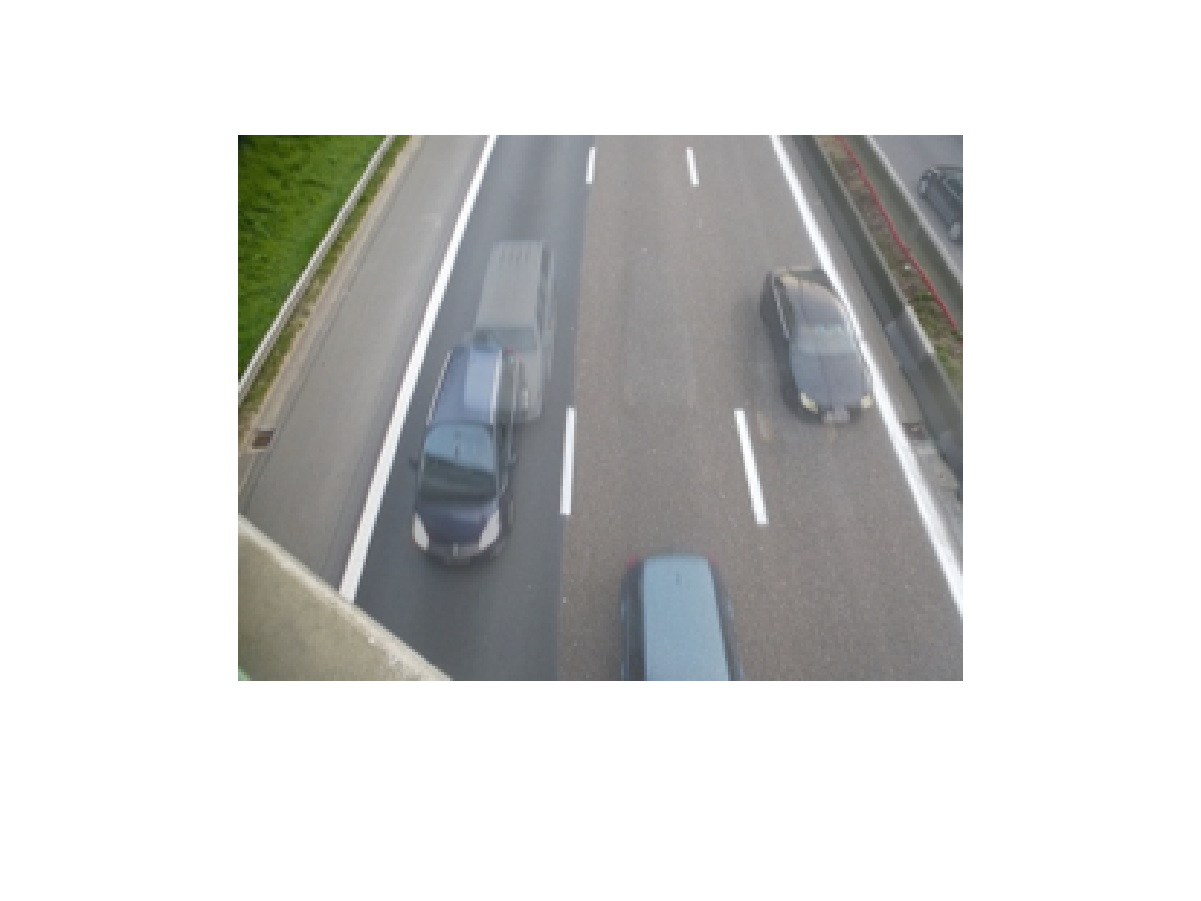
\includegraphics[{width= \textwidth}]{../Images/Camera/Autoroute/fg/a50/CamDeblurred-9.png}
\caption{}
\label{fig:UAut9}
\end{subfigure}
~
\begin{subfigure}{0.20\textwidth}
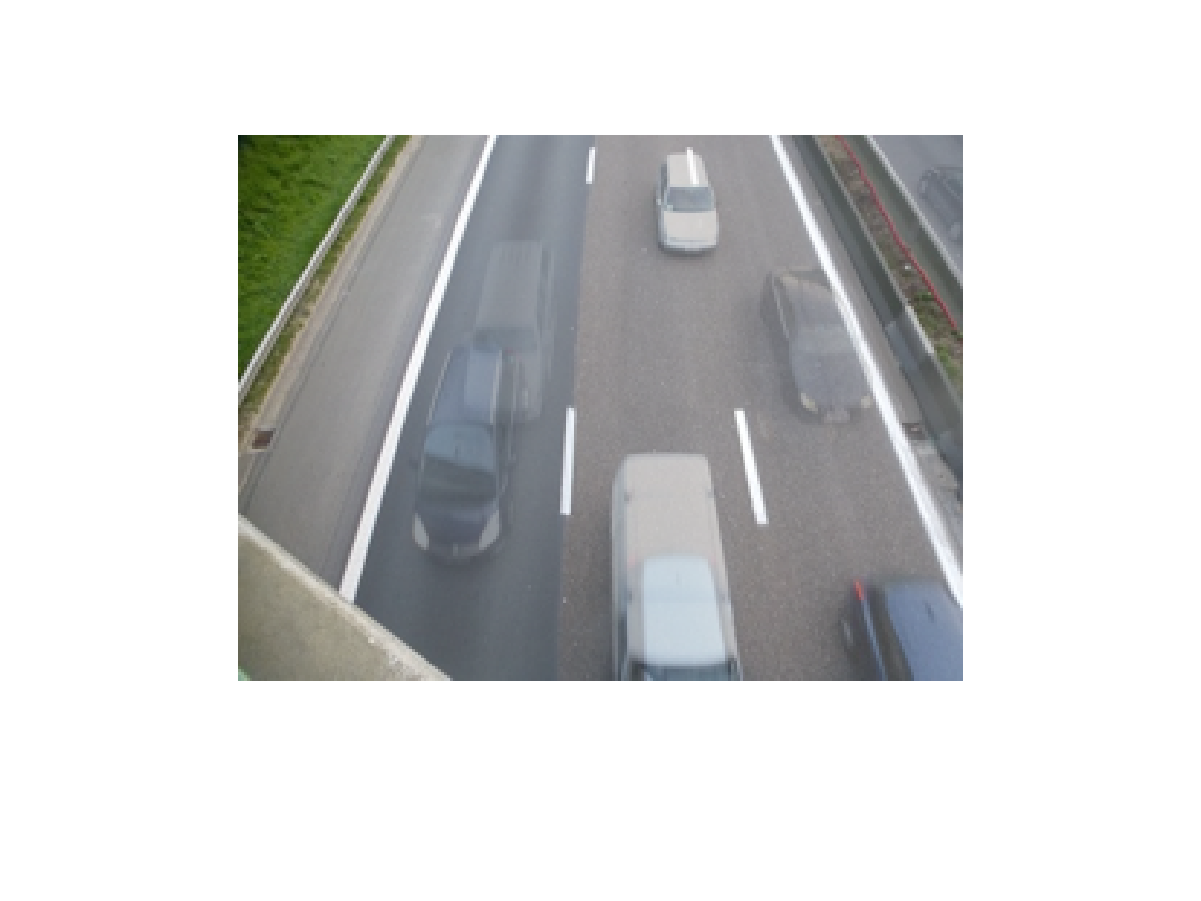
\includegraphics[{width= \textwidth}]{../Images/Camera/Autoroute/fg/a50/CamDeblurred-10.png}
\caption{}
\label{fig:UAut10}
\end{subfigure}
~
\begin{subfigure}{0.20\textwidth}
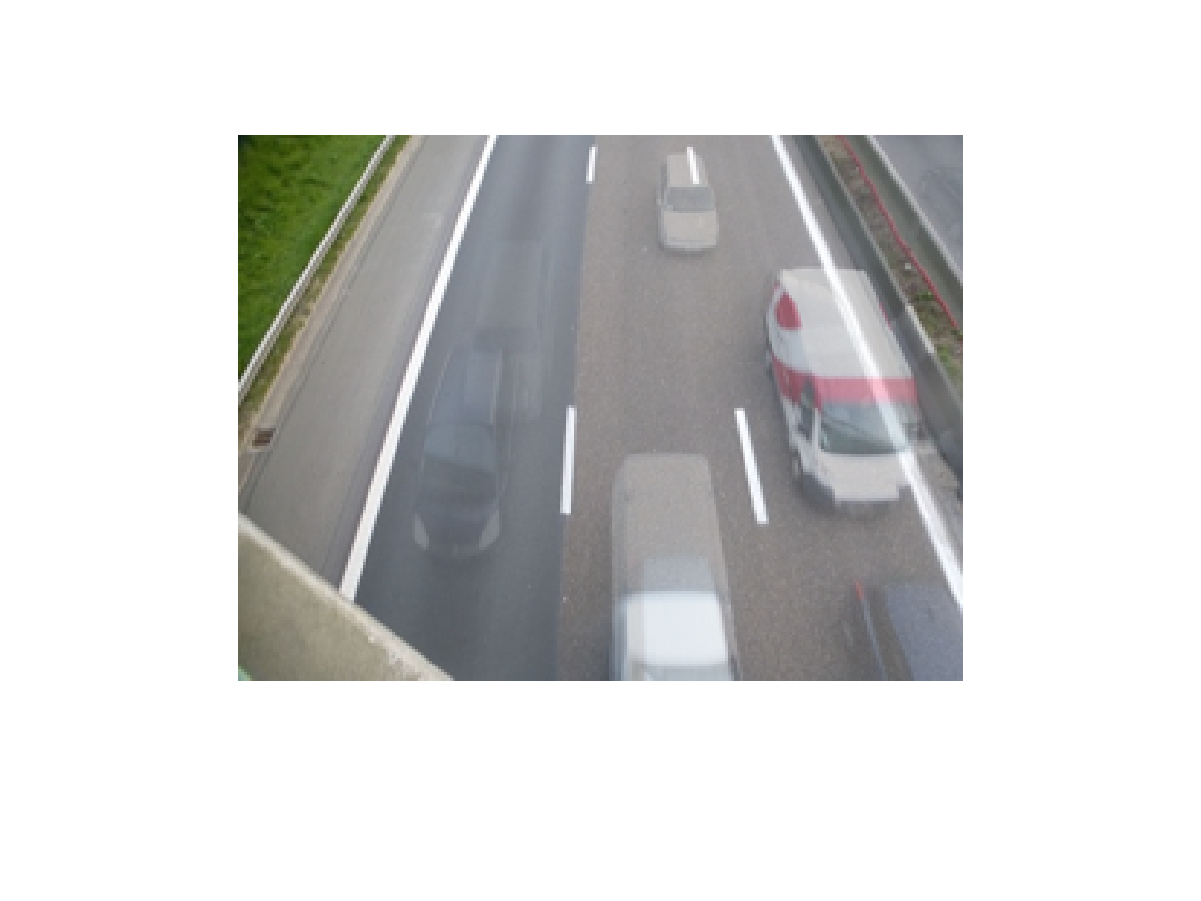
\includegraphics[{width= \textwidth}]{../Images/Camera/Autoroute/fg/a50/CamDeblurred-11.png}
\caption{}
\label{fig:UAut11}
\end{subfigure}
\caption{Udpade of the Background with $a=0.5$}
\label{fig:Udpade}
\end{figure}
\centering
\begin{subfigure}{0.20\textwidth}
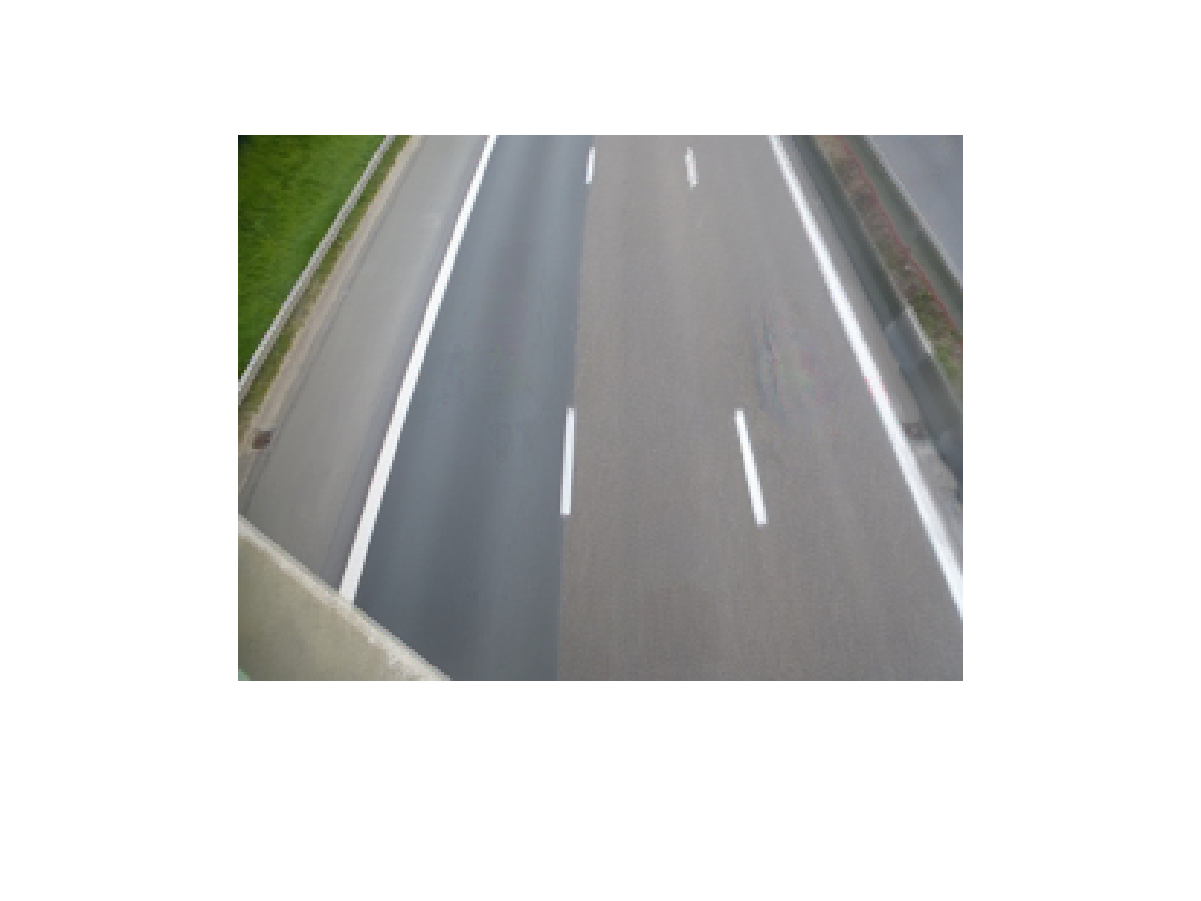
\includegraphics[width= \textwidth]{../Images/Camera/Autoroute/fg/a50/CamDeblurred-1.png}
\caption{}
\label{fig:UAut1}
\end{subfigure}
~
\begin{subfigure}{0.20\textwidth}
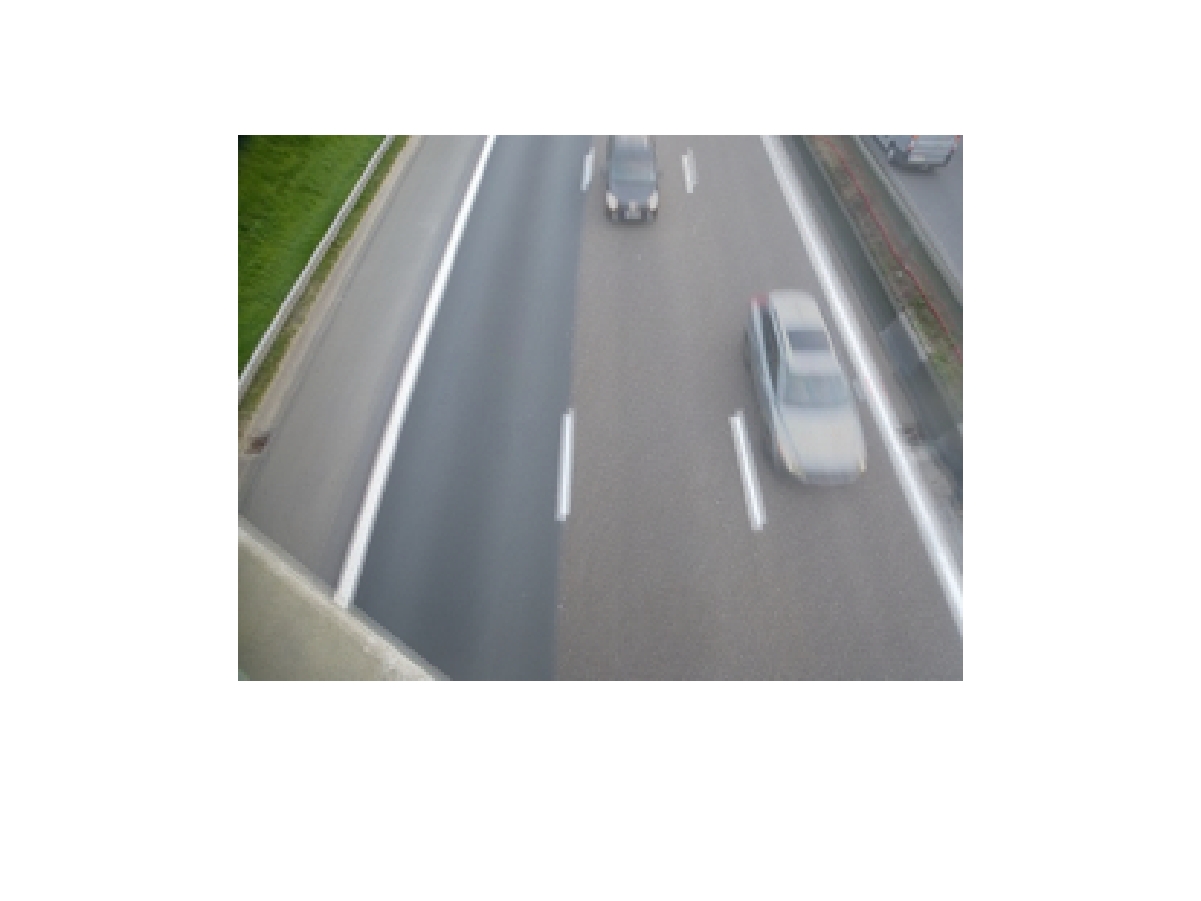
\includegraphics[{width= \textwidth}]{../Images/Camera/Autoroute/fg/a50/CamDeblurred-2.png}
\caption{}
\label{fig:UAut2}
\end{subfigure}
~
\begin{subfigure}{0.20\textwidth}
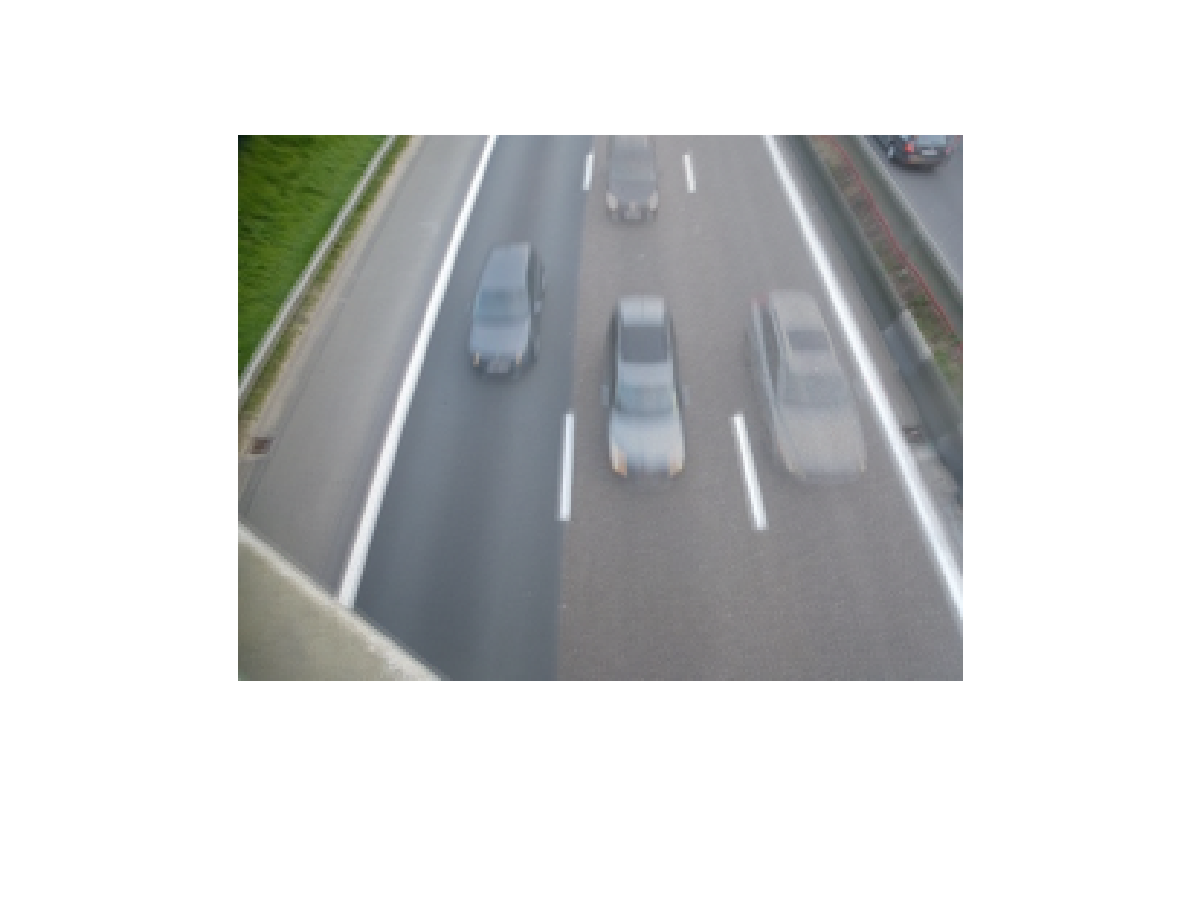
\includegraphics[{width= \textwidth}]{../Images/Camera/Autoroute/fg/a50/CamDeblurred-3.png}
\caption{}
\label{fig:UAut3}
\end{subfigure}
~
\begin{subfigure}{0.20\textwidth}
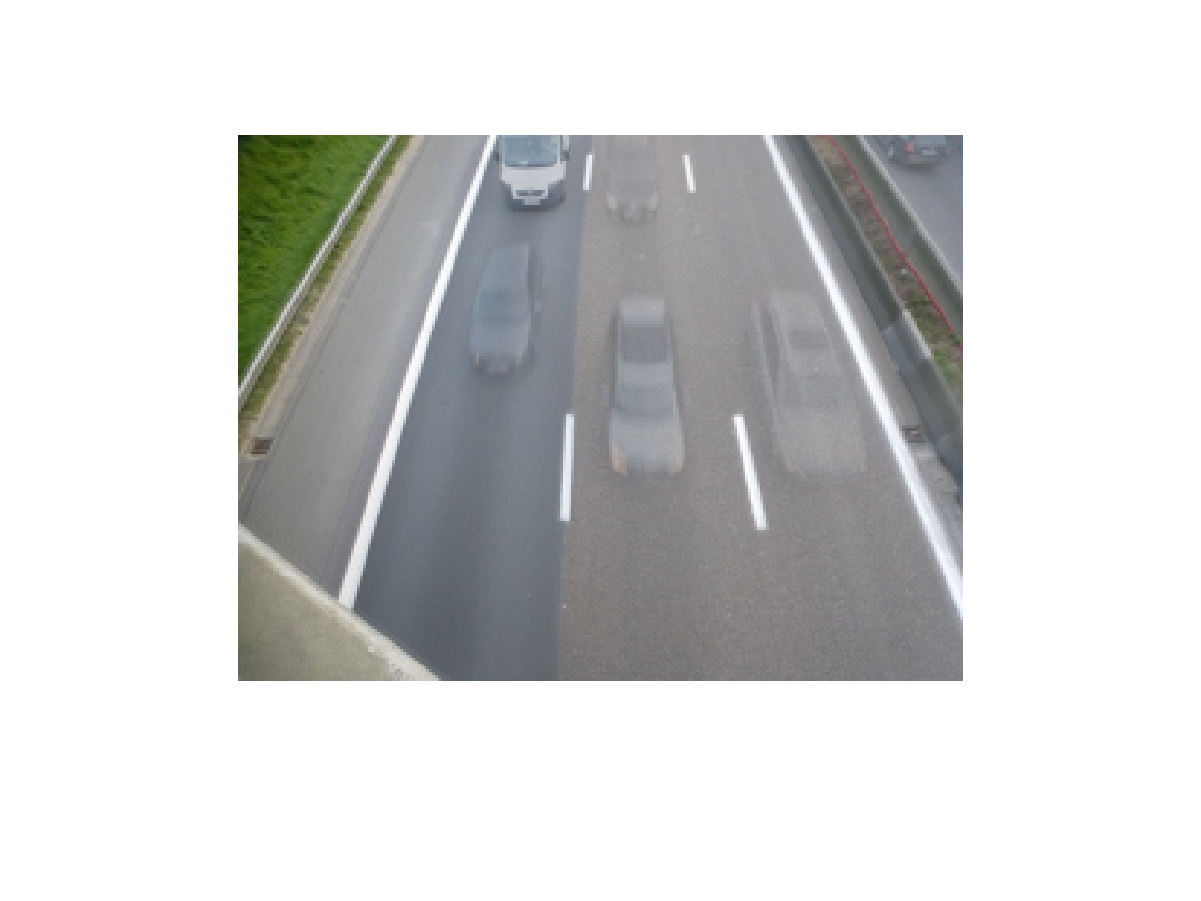
\includegraphics[{width= \textwidth}]{../Images/Camera/Autoroute/fg/a50/CamDeblurred-4.png}
\caption{}
\label{fig:UAut4}
\end{subfigure}
~
\begin{subfigure}{0.20\textwidth}
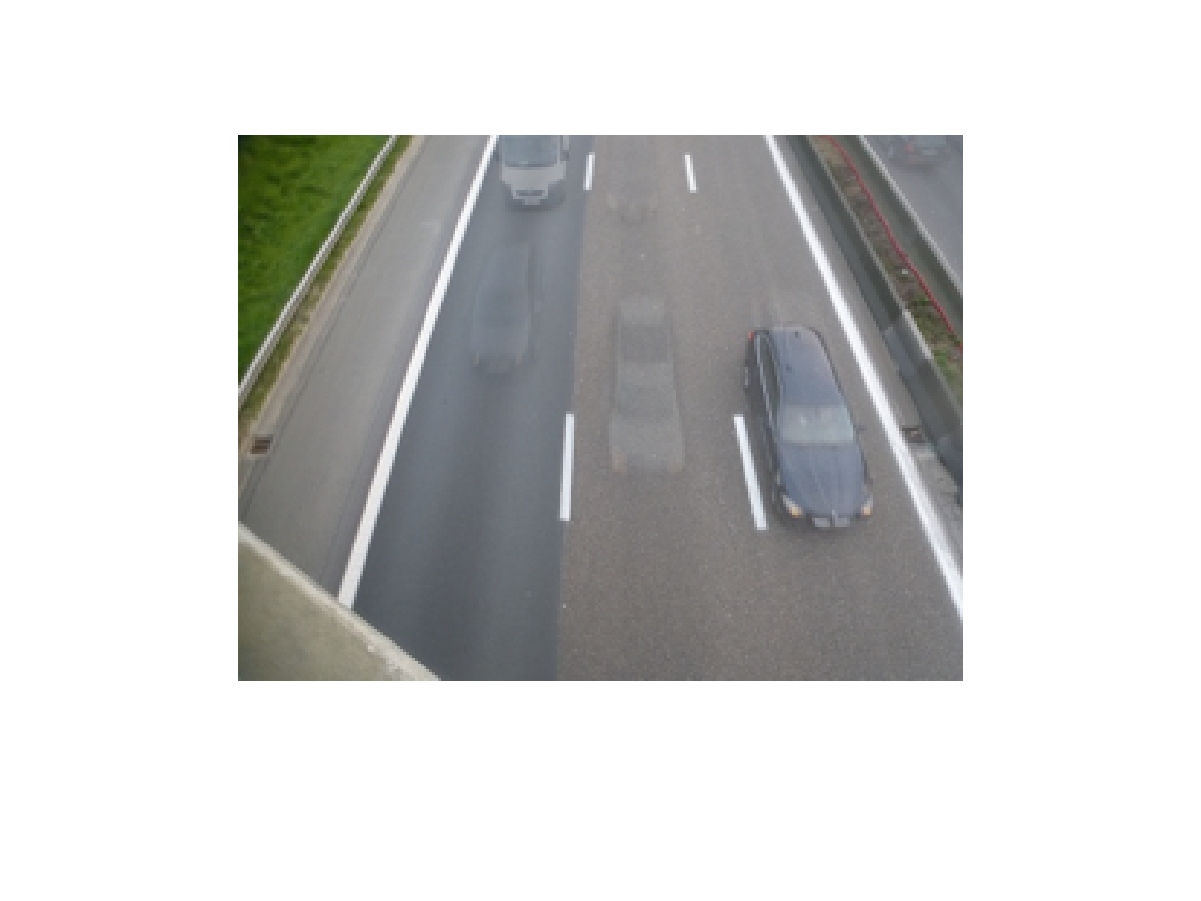
\includegraphics[{width= \textwidth}]{../Images/Camera/Autoroute/fg/a50/CamDeblurred-5.png}
\caption{}
\label{fig:UAut5}
\end{subfigure}
~
\begin{subfigure}{0.20\textwidth}
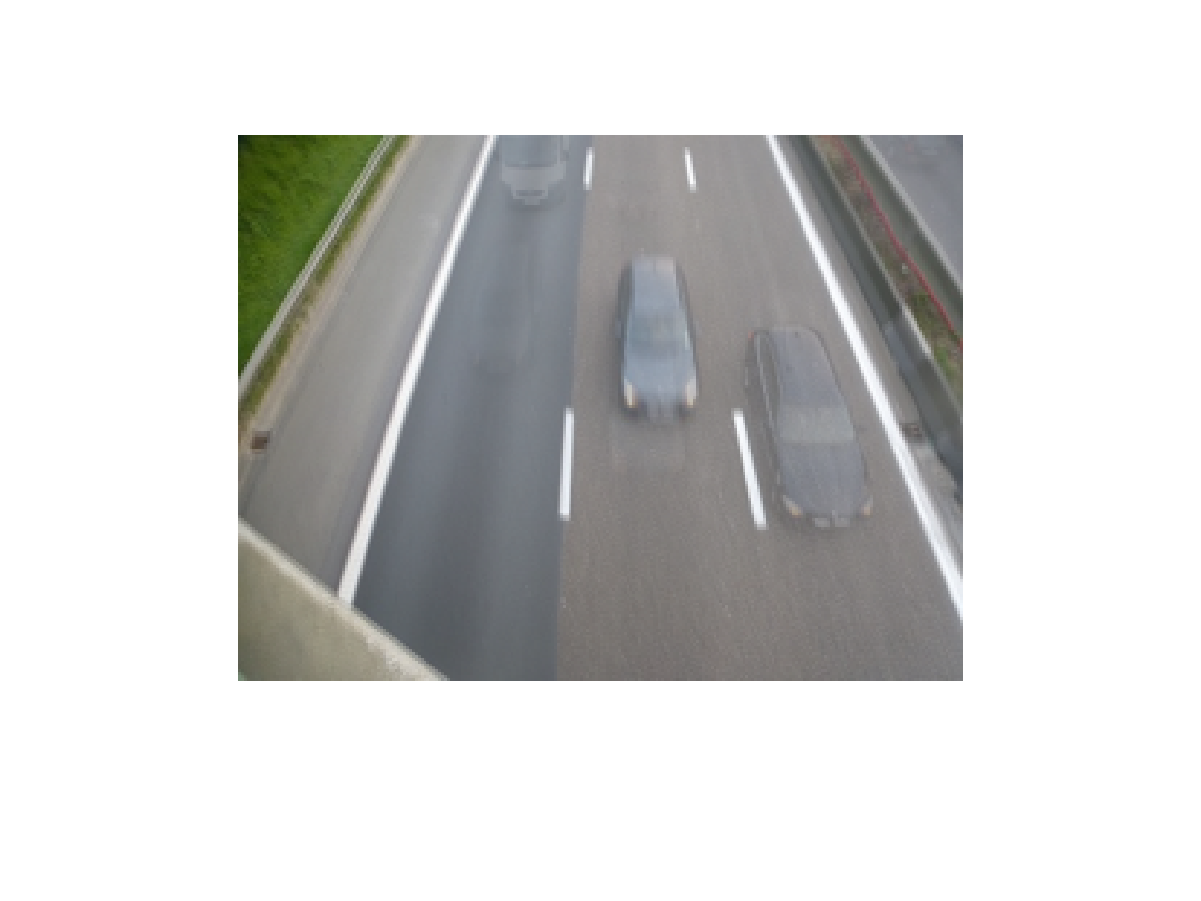
\includegraphics[{width= \textwidth}]{../Images/Camera/Autoroute/fg/a50/CamDeblurred-6.png}
\caption{}
\label{fig:UAut6}
\end{subfigure}
~
\begin{subfigure}{0.20\textwidth}
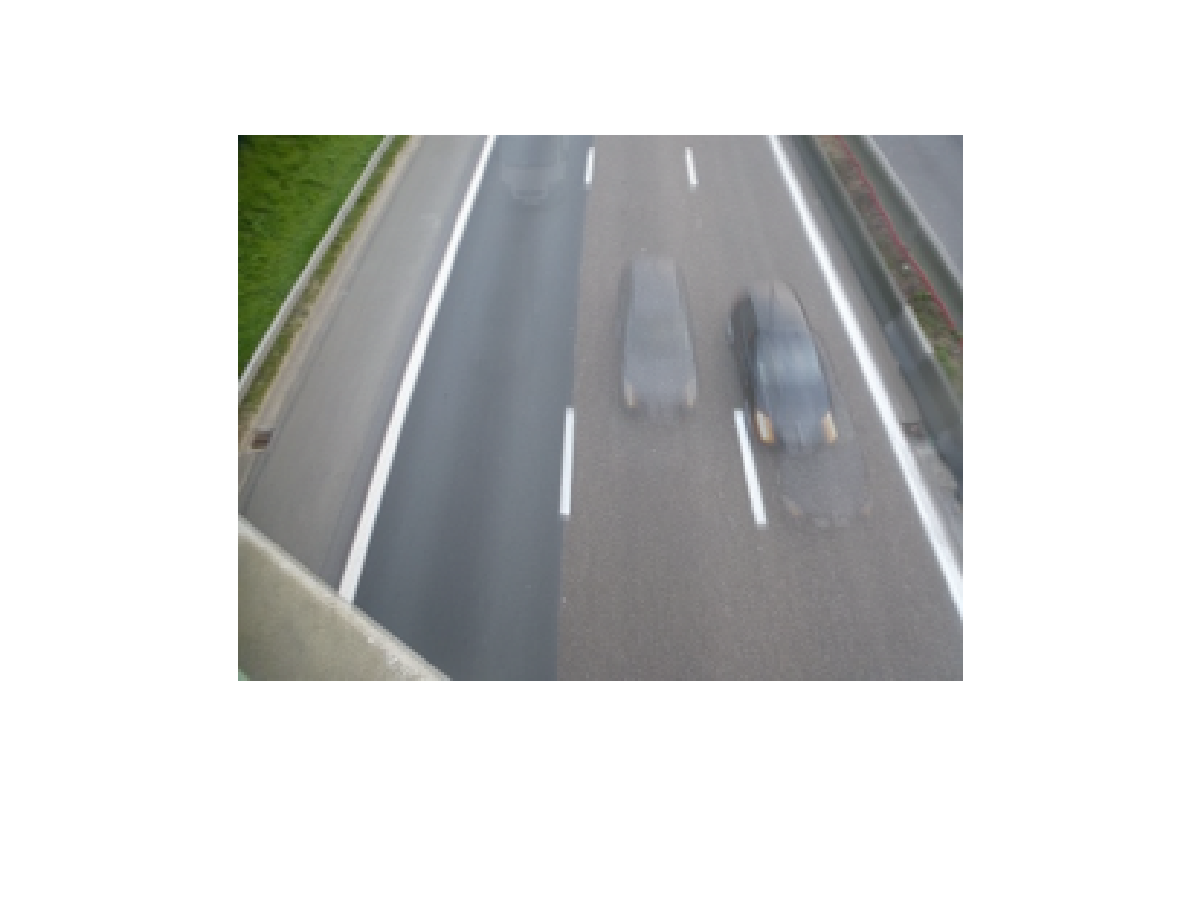
\includegraphics[{width= \textwidth}]{../Images/Camera/Autoroute/fg/a50/CamDeblurred-7.png}
\caption{}
\label{fig:UAut7}
\end{subfigure}
~
\begin{subfigure}{0.20\textwidth}
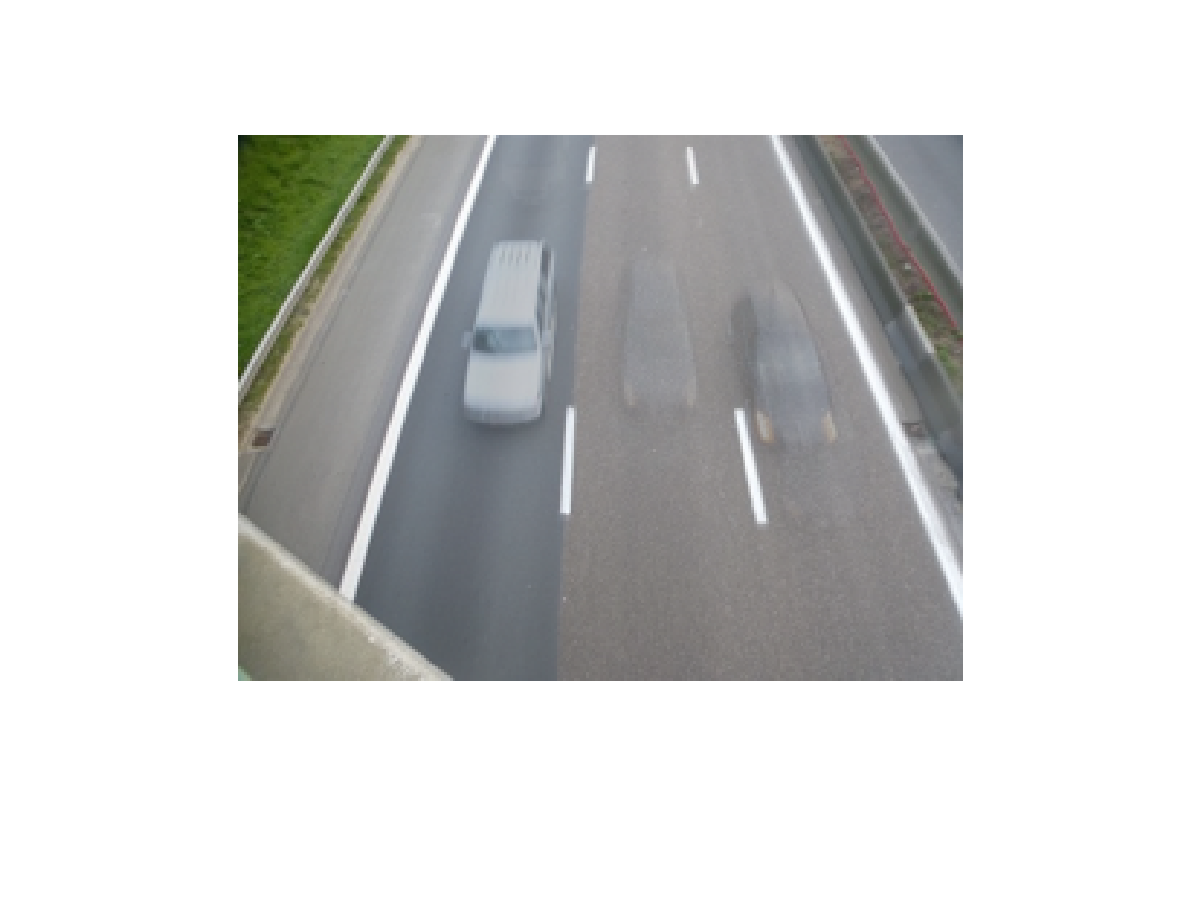
\includegraphics[{width= \textwidth}]{../Images/Camera/Autoroute/fg/a50/CamDeblurred-8.png}
\caption{}
\label{fig:UAut8}
\end{subfigure}
~
\begin{subfigure}{0.20\textwidth}
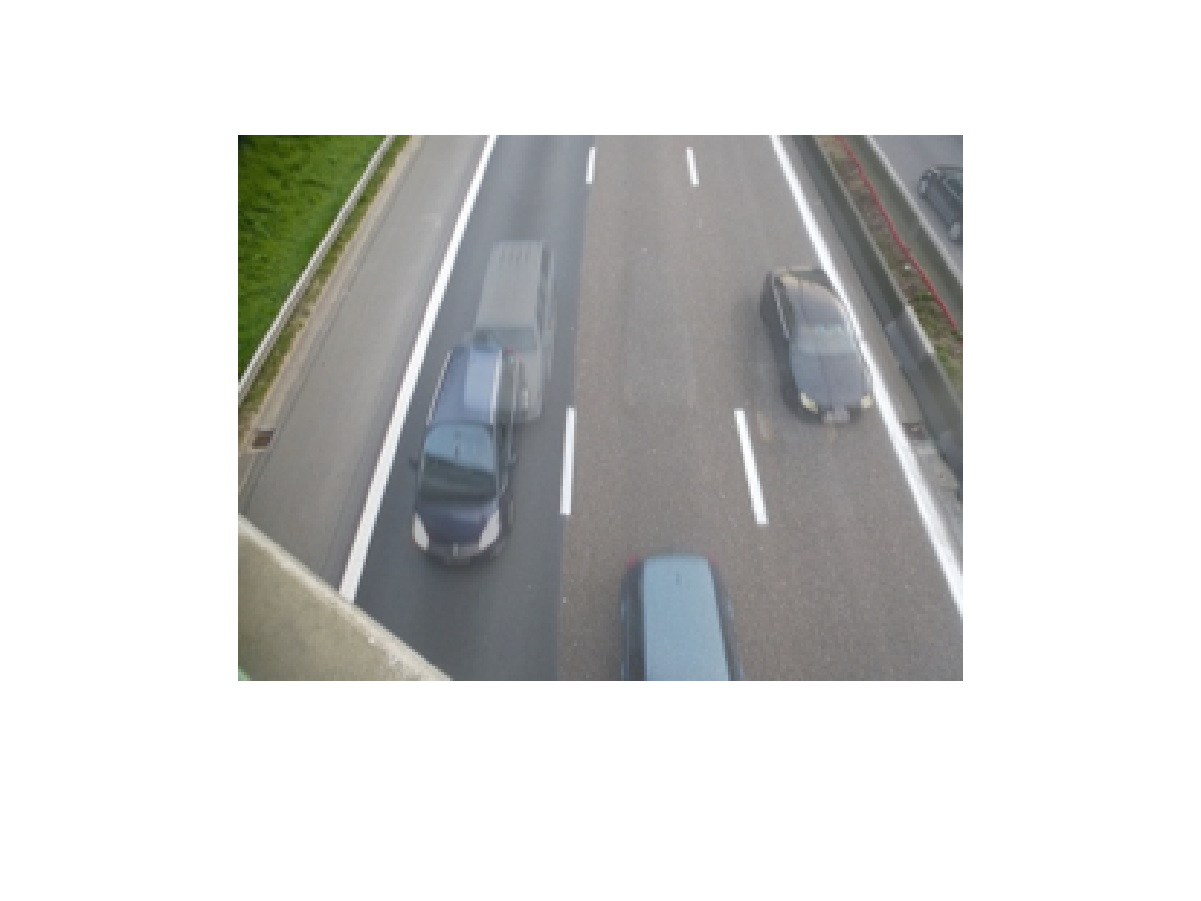
\includegraphics[{width= \textwidth}]{../Images/Camera/Autoroute/fg/a50/CamDeblurred-9.png}
\caption{}
\label{fig:UAut9}
\end{subfigure}
~
\begin{subfigure}{0.20\textwidth}
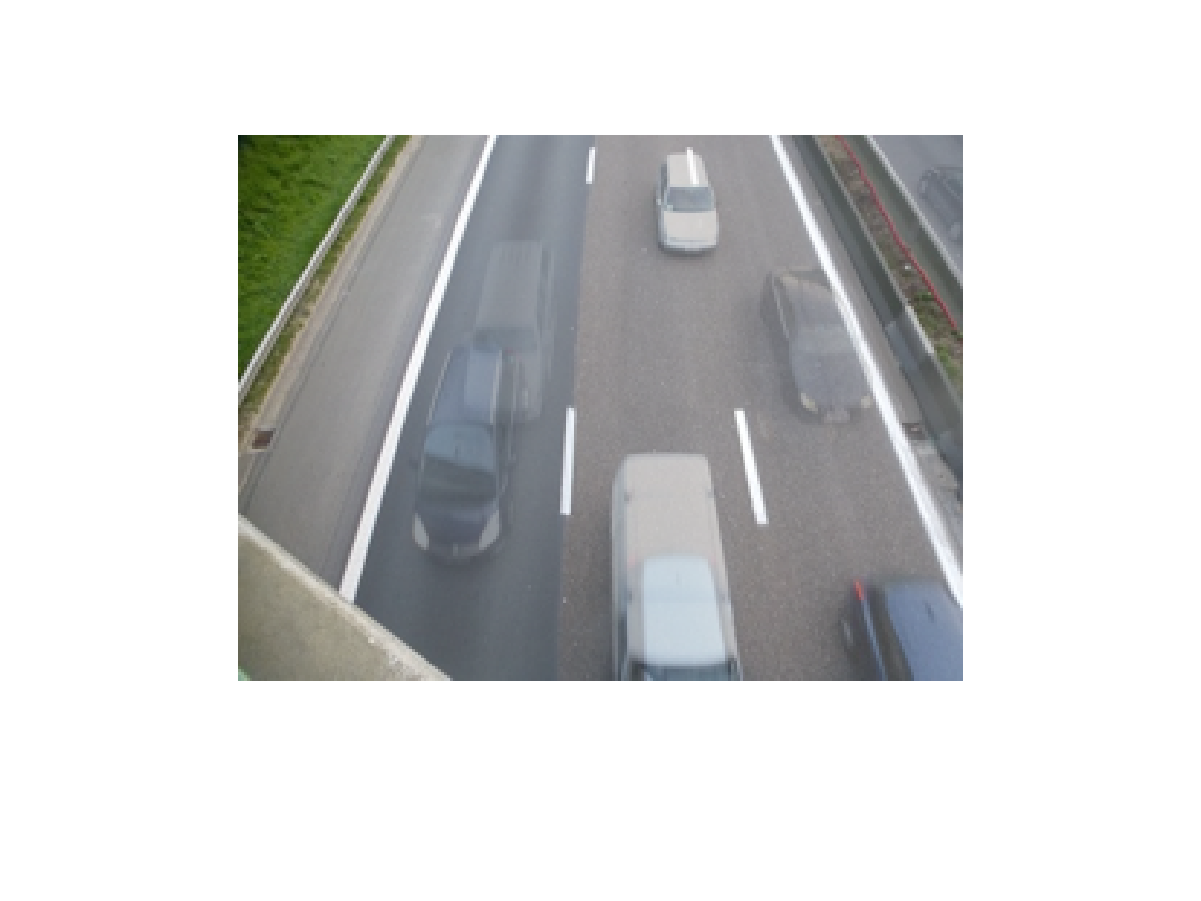
\includegraphics[{width= \textwidth}]{../Images/Camera/Autoroute/fg/a50/CamDeblurred-10.png}
\caption{}
\label{fig:UAut10}
\end{subfigure}
~
\begin{subfigure}{0.20\textwidth}
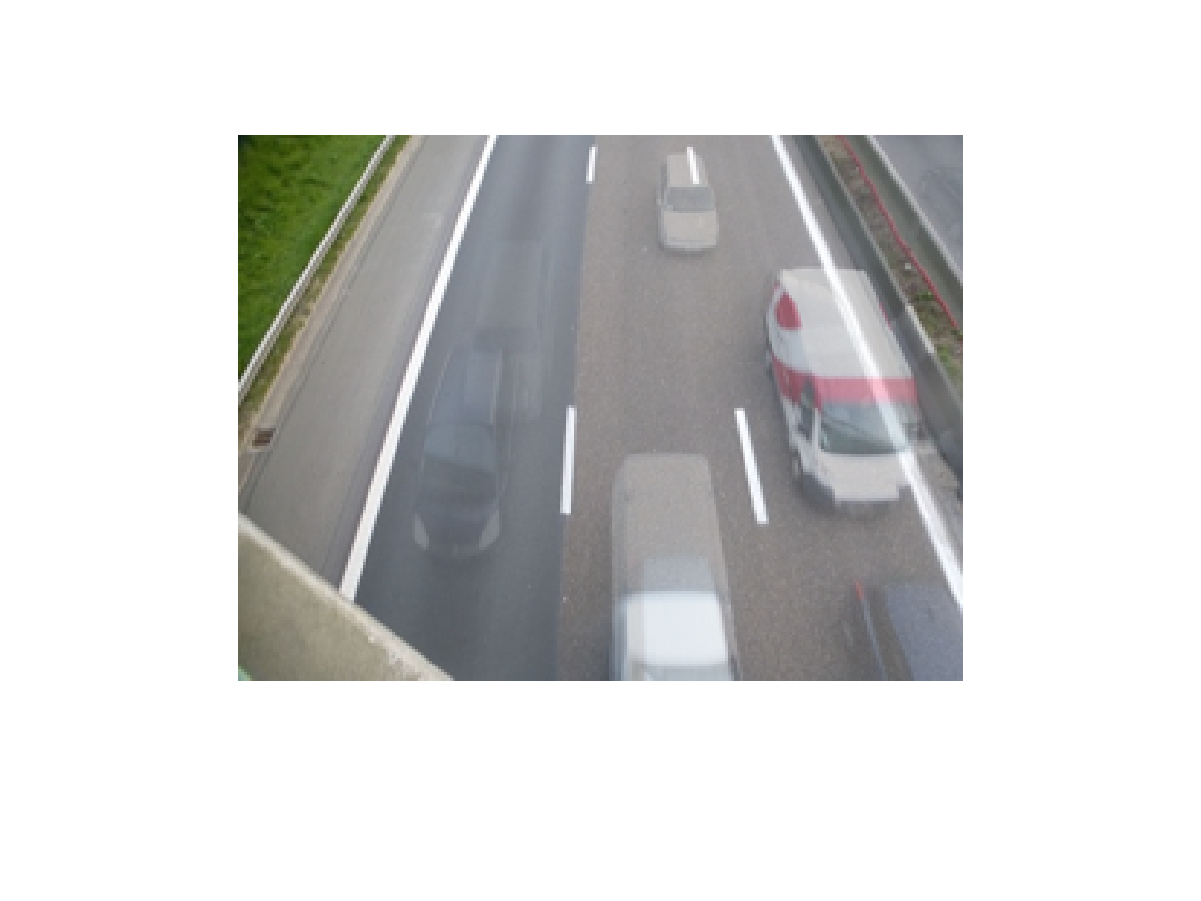
\includegraphics[{width= \textwidth}]{../Images/Camera/Autoroute/fg/a50/CamDeblurred-11.png}
\caption{}
\label{fig:UAut11}
\end{subfigure}
\caption{Udpade of the Background with $a=0.5$}
\label{fig:Udpade}
\end{figure}
	\end{enumerate}

\end{frame}

\section[Bonus Item]{Bonus Item : ``Real-time''}
\begin{frame}{PSF estimation}

The angle and length estimation are achieved with a $256 \times 256 $ pixels square. 
 
\begin{figure}[h]
\centering
\begin{subfigure}{0.4\textwidth}
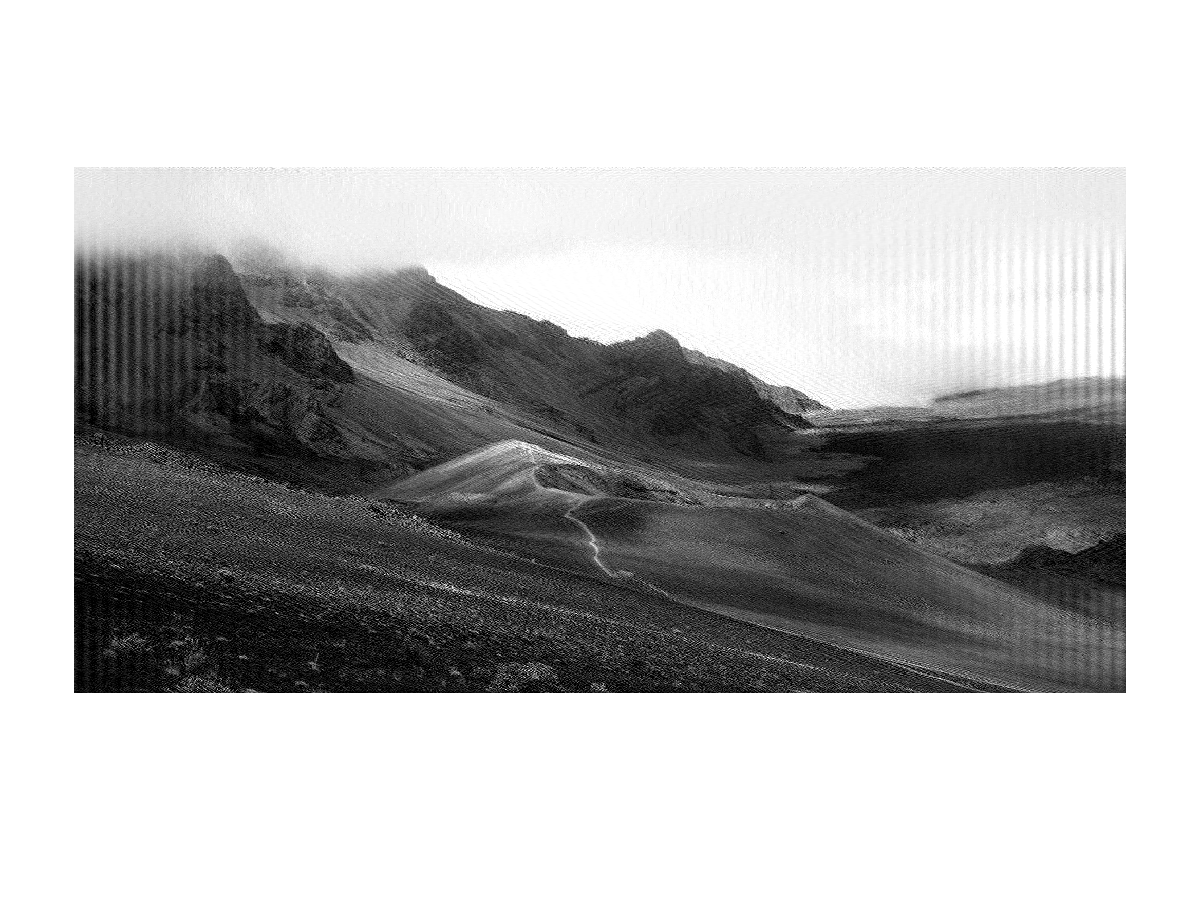
\includegraphics[width= \textwidth]{../Images/SagarShortEstimation.png}
\vspace{-20pt}
\caption{ $256\times 256$ centered crop of the picture. }
\label{fig:SagarShort}
\end{subfigure}
~
\begin{subfigure}{0.4\textwidth}
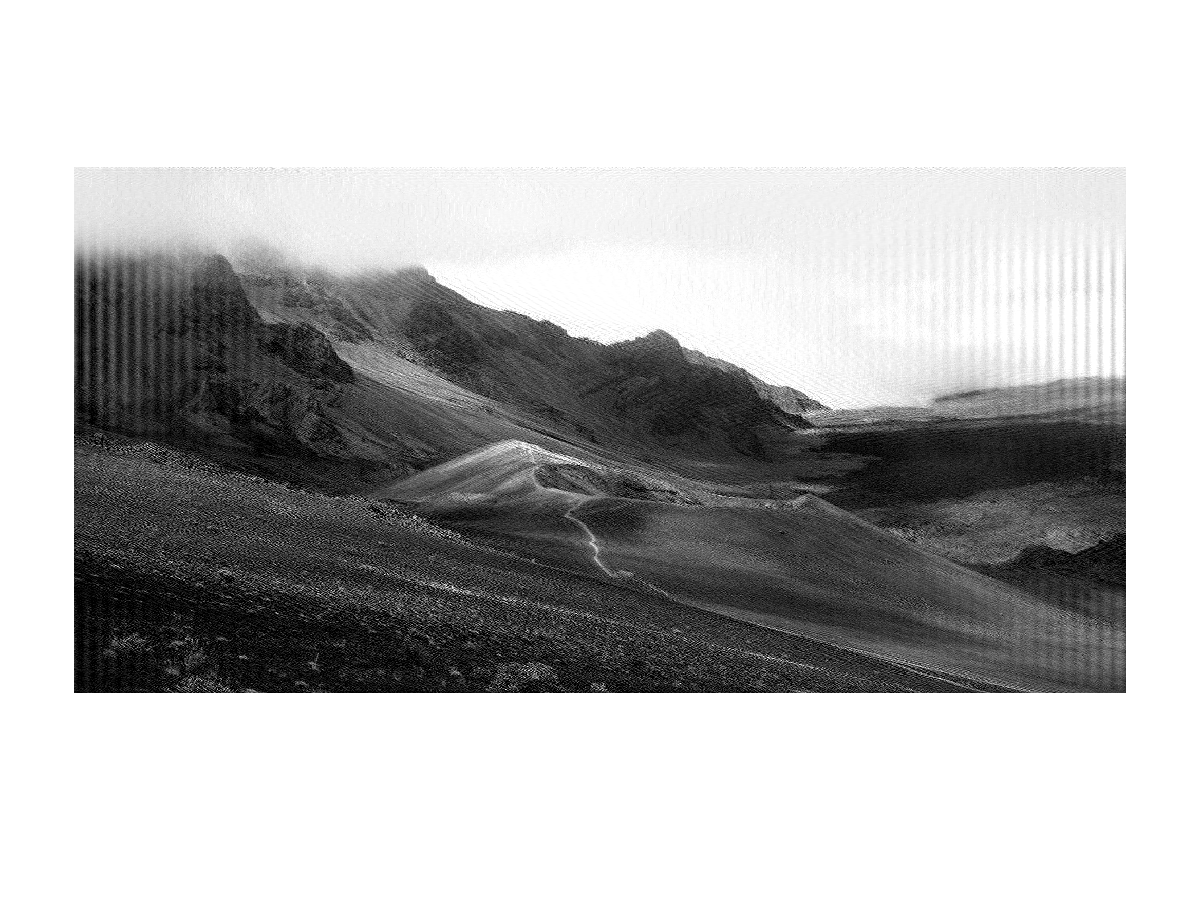
\includegraphics[{width= \textwidth}]{../Images/SagarLongEstimation.png}
\vspace{-20pt}
\caption{The whole image.}
\label{fig:SagarLong}
\end{subfigure}
\caption{Different matrix's size for the PSF estimation.}
\end{figure}
\end{frame}

\begin{frame}{Resizing}
 
Challenge : Artifacts may occur during the resizing process. 

\begin{figure}
\centering
\begin{subfigure}{0.4\textwidth}
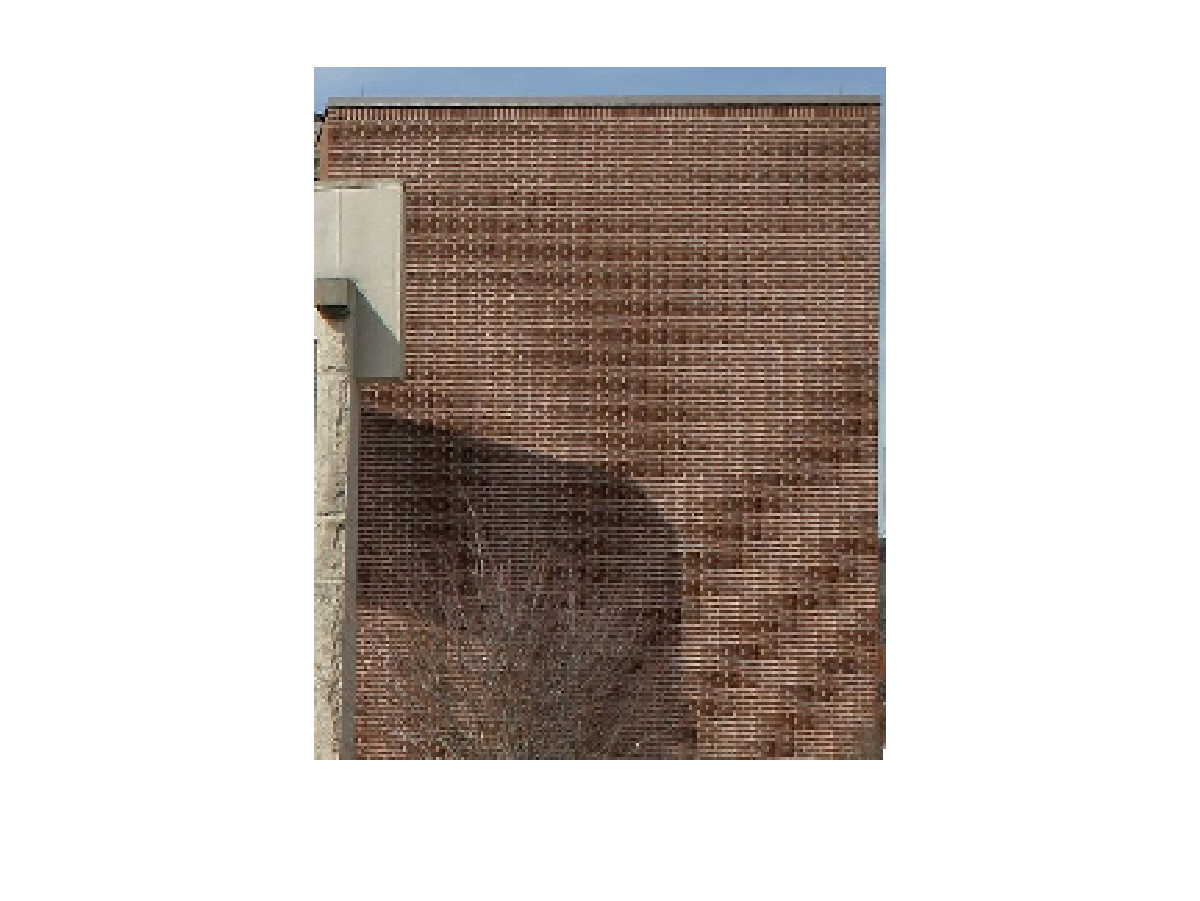
\includegraphics[width= \textwidth]{../Images/bricksCompressed.png}
\vspace{-20pt}
\caption{Nearest-Neighbor algorithm. }
\label{fig:bricksCompressed}
\end{subfigure}
~
\begin{subfigure}{0.4\textwidth}
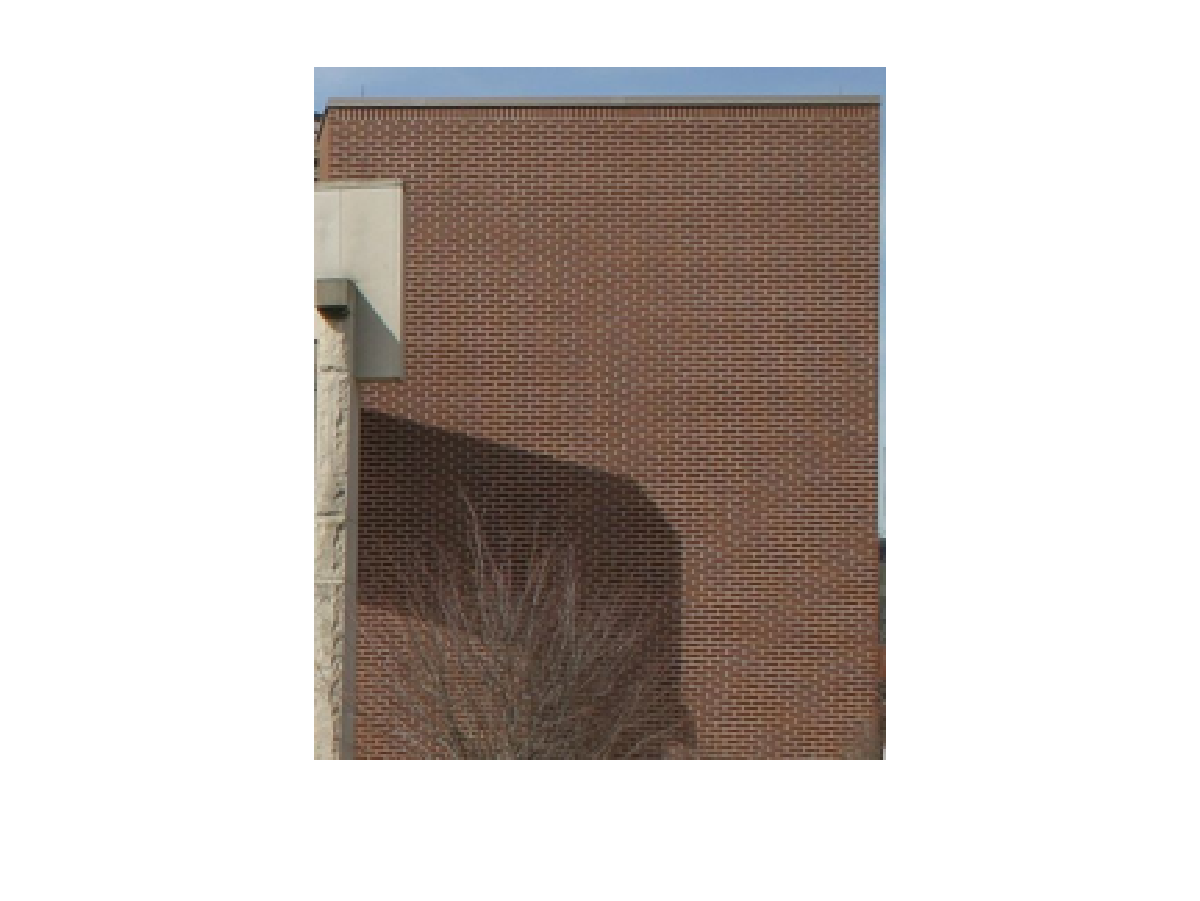
\includegraphics[width = \textwidth]{../Images/bricksLanczos.png}
\vspace{-20pt}
\caption{Lanczos2 algorithm.}
\label{fig:bricksLanczos}
\end{subfigure}
\caption{Picture resized using different algorithms}
\end{figure}

\end{frame}

\input{ComparisonResults/ComparisonResults}

We finally finished our image deblurring project and we have here presented our main results. Let's remember the main points of our project. 

After some time spent on understanding the problem, we wrote the mathematical model which enabled us to structure our ideas and identify the key challenges of deblurring. This model is written in chapter \ref{mathModel}. We decided to manage two cases : the train, i.e. a linear motion blur with an angle and the camera, i.e. a sharp background and a blurred foreground which we restrain to the same type of blur as in the train case. 

We then split our problem in three main parts : the estimation of the psf for the train, the deconvolution for the train and then the adaptation for the camera. 

Estimating the psf needs different values. The first one is the angle of the psf. To compute this angle, we implemented different methods, one using radon and the other using gabor, as explained in subsections \ref{subsec:Radon} and \ref{subsec:Gabor}. Then we estimated the length of the psf. To do this, we used a modified cepstrum as explained in subsection \ref{subsec:Cep}. This psf estimation gives accurate results most of the time even if for some pictures we don't get the exact psf. 

Once we had our estimated psf, we focused on the deconvolution. After a quick review of the simple inverse filter, we used three different algorithms for this deconvolution : Lucy-Richardson, Wiener and regularisation. Lucy-Richardson is based on a poisson distribution and on a fix point method for the iterations i order to converge to the MLE, as explained in subsection \ref{subsec:Lucy}. Wiener deconvolution gives the minimum mean-square error estimate of the initial image using an estimation of the noise's and image's power spectrum. The regularisation is based on an inverse filter to which was added a term.  This term penalizes the high frequencies and so the noise and avoid the problems experienced with the inverse filter. For further details, please refer to the subsections \ref{subsec:Wiener} and \ref{subsec:Reg}.

Besides these deconvolutions, we implemented some complementary treatments. Estimating the nsr required a smooth region. We wanted a mathematical criterion to compare the sharpness of different results for the same blurred image, we also managed the problem with the edges and some details with the colors, as written in section \ref{sec:CompTr}.


We then moved to the camera. The first aspect is to have a proper background without interference,such as  people walking in front of the camera for example. Then we can detect the foreground by comparing the new picture with the estimated background. We finally have to compute our psf based on the foreground only. All these aspects are explained in chapter \ref{chap:Camera}. 

The "real-time" was our bonus item. As exact real-time was difficult to achieve and we found it less interesting in the context of image deblurring than others aspects available to reduce the computation time we decide to implement an image resizing and a psf estimation on a smaller part of the image as described in section \ref{sec:RealTime}. 

Finally, in chapter \ref{chap:Comparison}, we test different aspects of our methods like the computation time, the quality of the psf estimation, and last but not least real images.  Some results were encouraging, some others less. We finally identify the main improvements that could be implemented for even better results.

 



\section{Quelques résolution avec PSF connue}

%\begin{figure}[!ht]
%  \centering
%  \begin{subfigure}[b]{0.45\textwidth}
%    \includegraphics[width=\textwidth]{../matlab/start-nonoise.png}
%    \caption{Image de départ}
%    \label{fig:start-nonoise}
%  \end{subfigure}
%  \begin{subfigure}[b]{0.45\textwidth}
%    \includegraphics[width=\textwidth]{../matlab/matb-nonoise.png}
%    \caption{Image flouté par matrice}
%    \label{fig:matb-nonoise}
%  \end{subfigure}%
%  \begin{subfigure}[b]{0.45\textwidth}
%    \includegraphics[width=\textwidth]{../matlab/psfb-nonoise.png}
%    \caption{Image floutée par PSF}
%    \label{fig:psfb-nonoise_explicite_lambda}
%  \end{subfigure}
%  \begin{subfigure}[b]{0.45\textwidth}
%    \includegraphics[width=\textwidth]{../matlab/direct-nonoise.png}
%    \caption{Image déflouté par méthode directe}
%    \label{fig:direct-nonoise}
%  \end{subfigure}
%  \begin{subfigure}[b]{0.45\textwidth}
%    \includegraphics[width=\textwidth]{../matlab/lucy-nonoise.png}
%    \caption{Image défloutée par Lucy-Richardson}
%    \label{fig:lucy-nonoise}
%  \end{subfigure}
%  \caption{Résultats pour une image sans noise}
%  \label{fig:nonoise}
%\end{figure}
%
%\begin{figure}[!ht]
%  \centering
%  \begin{subfigure}[b]{0.45\textwidth}
%    \includegraphics[width=\textwidth]{../matlab/start-noise-g10.png}
%    \caption{Image de départ}
%    \label{fig:start-noise-g10}
%  \end{subfigure}
%  \begin{subfigure}[b]{0.45\textwidth}
%    \includegraphics[width=\textwidth]{../matlab/matb-noise-g10.png}
%    \caption{Image flouté par matrice}
%    \label{fig:matb-noise-g10}
%  \end{subfigure}%
%  \begin{subfigure}[b]{0.45\textwidth}
%    \includegraphics[width=\textwidth]{../matlab/psfb-noise-g10.png}
%    \caption{Image floutée par PSF}
%    \label{fig:psfb-noise-g10_explicite_lambda}
%  \end{subfigure}
%  \begin{subfigure}[b]{0.45\textwidth}
%    \includegraphics[width=\textwidth]{../matlab/direct-noise-g10.png}
%    \caption{Image déflouté par méthode directe}
%    \label{fig:direct-noise-g10}
%  \end{subfigure}
%  \begin{subfigure}[b]{0.45\textwidth}
%    \includegraphics[width=\textwidth]{../matlab/lucy-noise-g10.png}
%    \caption{Image défloutée par Lucy-Richardson}
%    \label{fig:lucy-noise-g10}
%  \end{subfigure}
%  \caption{Résultats pour une image avec noise gaussien}
%  \label{fig:noise-g10}
%\end{figure}
%
%\begin{figure}[!ht]
%  \centering
%  \begin{subfigure}[b]{0.45\textwidth}
%    \includegraphics[width=\textwidth]{../matlab/start-noise-poisson.png}
%    \caption{Image de départ}
%    \label{fig:start-noise-poisson}
%  \end{subfigure}
%  \begin{subfigure}[b]{0.45\textwidth}
%    \includegraphics[width=\textwidth]{../matlab/matb-noise-poisson.png}
%    \caption{Image flouté par matrice}
%    \label{fig:matb-noise-poisson}
%  \end{subfigure}%
%  \begin{subfigure}[b]{0.45\textwidth}
%    \includegraphics[width=\textwidth]{../matlab/psfb-noise-poisson.png}
%    \caption{Image floutée par PSF}
%    \label{fig:psfb-noise-poisson_explicite_lambda}
%  \end{subfigure}
%  \begin{subfigure}[b]{0.45\textwidth}
%    \includegraphics[width=\textwidth]{../matlab/direct-noise-poisson.png}
%    \caption{Image déflouté par méthode directe}
%    \label{fig:direct-noise-poisson}
%  \end{subfigure}
%  \begin{subfigure}[b]{0.45\textwidth}
%    \includegraphics[width=\textwidth]{../matlab/lucy-noise-poisson.png}
%    \caption{Image défloutée par Lucy-Richardson}
%    \label{fig:lucy-noise-poisson}
%  \end{subfigure}
%  \caption{Résultats pour une image avec noise poisson}
%  \label{fig:noise-poisson}
%\end{figure}

\bibliographystyle{plain}
\bibliography{biblio}

\end{document}
